\documentclass[10pt,aps,pra,twocolumn,showpacs,superscriptaddress,nobalancelastpage,notitlepage,nofootinbib,longbibliography]{revtex4-2}

%\bibliographystyle{apsrev4-2-titles}
\bibliographystyle{ieeetr}
\usepackage[usenames,dvipsnames]{xcolor}

\usepackage{cancel}
\usepackage{amsfonts,amsmath,amssymb}
\usepackage{calc}
\usepackage[english]{babel}
\usepackage[normalem]{ulem}
\usepackage{hyperref}
\let\proof\relax 
\let\endproof\relax
\usepackage{amsthm}
\usepackage{graphicx}

\usepackage{quiver}

\usepackage[linesnumbered,noend]{algorithm2e}

\usepackage{subcaption,caption}
\usepackage{epsfig}
%\usepackage{dirtytalk}
\usepackage{ulem}
\usepackage{tikz}
\usepackage{mathrsfs}
\usepackage{bbold}             % This package was used to write the one with double bars 

\usepackage{soul}

\usepackage{pgfplots}

\pgfplotsset{compat = newest}

\usepackage{bm}
\usetikzlibrary{shapes,arrows}
\usetikzlibrary{matrix}
\usetikzlibrary{calc,patterns,angles,quotes,arrows,automata}
\graphicspath{ {./imgs/}}

% \usepackage{natbib}
% \usepackage{float}
% \usepackage{widetext}

% \usepackage{listings}

% \usepackage{mdframed}

%\theoremstyle{definition}
\makeatother
\usepackage{thmtools}
%\usepackage[framemethod=TikZ]{mdframed}

\def \colal {20}

\declaretheorem[mdframed={linewidth=0pt,
                            backgroundcolor=ForestGreen!\colal, 
                            innertopmargin=-2pt, innerleftmargin=0pt, leftmargin=0pt,
                            innerrightmargin=0pt},
                            %shaded={bgcolor=ForestGreen!\colal}, 
                            style=definition, name=Definition]{definition}
\declaretheorem[mdframed={linewidth=0pt,
                            backgroundcolor=ForestGreen!\colal, 
                            innertopmargin=-2pt, innerleftmargin=0pt, leftmargin=0pt,
                            innerrightmargin=0pt},
                            %shaded={bgcolor=ForestGreen!\colal}, 
                            style=definition, name=Assumption]{assumption}
%\declaretheorem[shaded={bgcolor=ForestGreen!\colal}, style=definition, 
%name=Definition, numbered=no]{definition*}
\declaretheorem[mdframed={linewidth=0pt,
                            backgroundcolor=RawSienna!\colal, 
                            innertopmargin=-2pt, innerleftmargin=0pt, leftmargin=0pt,
                            innerrightmargin=0pt},
                            %shaded={bgcolor=RawSienna!\colal}, 
                            name=Theorem]{theorem}
%\declaretheorem[shaded={bgcolor=RawSienna!\colal}, name=Theorem, numbered=no]{theorem*}
\declaretheorem[mdframed={linewidth=0pt,
                            backgroundcolor=RawSienna!\colal, 
                            innertopmargin=-2pt, innerleftmargin=0pt, leftmargin=0pt,
                            innerrightmargin=0pt},
                            %shaded={bgcolor=RawSienna!\colal}, 
                            name=Lemma]{lemma}
\declaretheorem[mdframed={linewidth=0pt,
                            backgroundcolor=RawSienna!\colal, 
                            innertopmargin=-2pt, innerleftmargin=0pt, leftmargin=0pt,
                            innerrightmargin=0pt},
                            %shaded={bgcolor=RawSienna!\colal}, 
                            name=Proposition]{proposition}
\declaretheorem[mdframed={linewidth=0pt,
                            backgroundcolor=RawSienna!\colal, 
                            innertopmargin=-2pt, innerleftmargin=0pt, leftmargin=0pt,
                            innerrightmargin=0pt},
                            %shaded={bgcolor=RawSienna!\colal}, 
                            name=Corollary]{corollary}
\declaretheorem[mdframed={linewidth=0pt,
                            backgroundcolor=RawSienna!\colal, 
                            innertopmargin=-2pt, innerleftmargin=0pt, leftmargin=0pt,
                            innerrightmargin=0pt},
                            %shaded={bgcolor=RawSienna!\colal}, 
                            name=Conjecture]{conjecture}
%\declaretheorem[mdframed={linewidth=0pt,
%                            backgroundcolor=RawSienna!\colal, 
%                            innertopmargin=-2pt, innerleftmargin=0pt, leftmargin=0pt,
%                            innerrightmargin=0pt},
%                            shaded={bgcolor=RawSienna!5}, name=Proof]{Proof}

\declaretheorem[mdframed={linewidth=0pt,
                            backgroundcolor=TealBlue!\colal,
                            innertopmargin=-2pt, innerleftmargin=0pt,
                            innerrightmargin=0pt}, 
                            style=definition, name=Example]{example}
\declaretheorem[mdframed={linewidth=0pt,
                            backgroundcolor=NavyBlue!\colal, 
                            innertopmargin=-2pt, innerleftmargin=0pt, leftmargin=0pt,
                            innerrightmargin=0pt},
                            %shaded={bgcolor=NavyBlue!\colal}, 
                            style=definition, numbered=no, name=Remark]{remark}
\declaretheorem[mdframed={linewidth=0pt,
                            backgroundcolor=WildStrawberry!\colal, 
                            innertopmargin=-2pt, innerleftmargin=0pt, leftmargin=0pt,
                            innerrightmargin=0pt},
                            %shaded={bgcolor=WildStrawberry!\colal}, 
                            style=definition, name=Problem]{problem}


\declaretheorem[mdframed={linewidth=0pt,
                            backgroundcolor=RawSienna!10, 
                            innertopmargin=-2pt, innerleftmargin=0pt, leftmargin=0pt,
                            innerrightmargin=0pt,}, 
                            style=definition,
                            numbered=no,qed=\qedsymbol, name=Proof]{replacementproof}
                            
\declaretheorem[mdframed={linewidth=0pt,
                            backgroundcolor=Cyan!\colal, 
                            innertopmargin=-2pt, innerleftmargin=0pt, leftmargin=0pt,
                            innerrightmargin=0pt},
                            %shaded={bgcolor=NavyBlue!\colal}, 
                            style=definition, numbered=no, name=Comment]{comment}
                            
\declaretheorem[mdframed={linewidth=0pt,
                            backgroundcolor=Mulberry!\colal, 
                            innertopmargin=-2pt, innerleftmargin=0pt, leftmargin=0pt,
                            innerrightmargin=0pt},
                            %shaded={bgcolor=NavyBlue!\colal}, 
                            style=definition, numbered=no, name=Comment]{classicalcomment}

\renewenvironment{proof}[1][\proofname]{
\ifnum\pdfstrcmp{#1}{\proofname}=0
  \replacementproof[ ]
\else
  \replacementproof[#1]
\fi
}{\endreplacementproof}

% \newcommand{\OneColumn}{
% \begingroup
% \let\clearpage\relax
% \onecolumn
% \endgroup}

% \newcommand{\TwoColumn}{
% \begingroup
% \let\clearpage\relax
% \twocolumn
% \endgroup}

\RestyleAlgo{ruled}
\SetKwInOut{Input}{Input}
\SetKwInOut{Output}{Output}
\SetKwInOut{Parameters}{Parameters}
\SetKwIF{If}{ElseIf}{Else}{if}{:}{else if}{else}{endif}

% ---------------------- Calligrapic
\newcommand{\Ac}{\mathcal{A}}
\newcommand{\Bc}{\mathcal{B}}
\newcommand{\Cc}{\mathcal{C}}
\newcommand{\Dc}{\mathcal{D}}
\newcommand{\Ec}{\mathcal{E}}
\newcommand{\Fc}{\mathcal{F}}
\newcommand{\Gc}{\mathcal{G}}
\newcommand{\Hc}{\mathcal{H}}
\newcommand{\Ic}{\mathcal{I}}
\newcommand{\Jc}{\mathcal{J}}
\newcommand{\Kc}{\mathcal{K}}
\newcommand{\Lc}{\mathcal{L}}
\newcommand{\Mc}{\mathcal{M}}
\newcommand{\Nc}{\mathcal{N}}
\newcommand{\Oc}{\mathcal{O}}
\newcommand{\Pc}{\mathcal{P}}
\newcommand{\Qc}{\mathcal{Q}}
\newcommand{\Rc}{\mathcal{R}}
\newcommand{\Sc}{\mathcal{S}}
\newcommand{\Tc}{\mathcal{T}}
\newcommand{\Uc}{\mathcal{U}}
\newcommand{\Vc}{\mathcal{V}}
\newcommand{\Wc}{\mathcal{W}}
\newcommand{\Xc}{\mathcal{X}}
\newcommand{\Yc}{\mathcal{Y}}
\newcommand{\Zc}{\mathcal{Z}}

% -------------------------- Script
\newcommand{\As}{\mathscr{A}}
\newcommand{\Bs}{\mathscr{B}}
\newcommand{\Cs}{\mathscr{C}}
\newcommand{\Ds}{\mathscr{D}}
\newcommand{\Es}{\mathscr{EL}}
\newcommand{\Fs}{\mathscr{F}}
\newcommand{\Gs}{\mathscr{G}}
\newcommand{\Hs}{\mathscr{H}}
\newcommand{\Is}{\mathscr{I}}
\newcommand{\Js}{\mathscr{J}}
\newcommand{\Ks}{\mathscr{K}}
\newcommand{\Ls}{\mathscr{L}}
\newcommand{\Ms}{\mathscr{M}}
\newcommand{\Ns}{\mathscr{N}}
\newcommand{\Os}{\mathscr{O}}
\newcommand{\Ps}{\mathscr{P}}
\newcommand{\Qs}{\mathscr{Q}}
\newcommand{\Rs}{\mathscr{R}}
\newcommand{\Ss}{\mathscr{S}}
\newcommand{\Ts}{\mathscr{T}}
\newcommand{\Us}{\mathscr{U}}
\newcommand{\Vs}{\mathscr{V}}
\newcommand{\Ws}{\mathscr{W}}
\newcommand{\Xs}{\mathscr{X}}
\newcommand{\Ys}{\mathscr{Y}}
\newcommand{\Zs}{\mathscr{Z}}

% -------------------------- Bold
\newcommand{\Ab}{\mathbb{A}}
\newcommand{\Bb}{\mathbb{B}}
\newcommand{\Cb}{\mathbb{C}}
\newcommand{\Db}{\mathbb{D}}
\newcommand{\Eb}{\mathbb{E}}
\newcommand{\Fb}{\mathbb{F}}
\newcommand{\Gb}{\mathbb{G}}
\newcommand{\Hb}{\mathbb{H}}
\newcommand{\Ib}{\mathbb{I}}
\newcommand{\Jb}{\mathbb{J}}
\newcommand{\Kb}{\mathbb{K}}
\newcommand{\Lb}{\mathbb{L}}
\newcommand{\Mb}{\mathbb{M}}
\newcommand{\Nb}{\mathbb{N}}
\newcommand{\Ob}{\mathbb{O}}
\newcommand{\Pb}{\mathbb{P}}
\newcommand{\Qb}{\mathbb{Q}}
\newcommand{\Rb}{\mathbb{R}}
\newcommand{\Sb}{\mathbb{S}}
\newcommand{\Tb}{\mathbb{T}}
\newcommand{\Ub}{\mathbb{U}}
\newcommand{\Vb}{\mathbb{V}}
\newcommand{\Wb}{\mathbb{W}}
\newcommand{\Xb}{\mathbb{X}}
\newcommand{\Yb}{\mathbb{Y}}
\newcommand{\Zb}{\mathbb{Z}}

% ------------------------- Fraktur
\newcommand{\Af}{\mathfrak{A}}
\newcommand{\Bf}{\mathfrak{B}}
\newcommand{\Cf}{\mathfrak{C}}
\newcommand{\Df}{\mathfrak{D}}
\newcommand{\Ef}{\mathfrak{E}}
\newcommand{\Ff}{\mathfrak{F}}
\newcommand{\Gf}{\mathfrak{G}}
\newcommand{\Hf}{\mathfrak{H}}
\newcommand{\Ifr}{\mathfrak{I}}
\newcommand{\Jf}{\mathfrak{J}}
\newcommand{\Kf}{\mathfrak{K}}
\newcommand{\Lf}{\mathfrak{L}}
\newcommand{\Mf}{\mathfrak{M}}
\newcommand{\Nf}{\mathfrak{N}}
\newcommand{\Of}{\mathfrak{O}}
\newcommand{\Pf}{\mathfrak{P}}
\newcommand{\Qf}{\mathfrak{Q}}
\newcommand{\Rf}{\mathfrak{R}}
\newcommand{\Sf}{\mathfrak{S}}
\newcommand{\Tf}{\mathfrak{T}}
\newcommand{\Uf}{\mathfrak{U}}
\newcommand{\Vf}{\mathfrak{V}}
\newcommand{\Wf}{\mathfrak{W}}
\newcommand{\Xf}{\mathfrak{X}}
\newcommand{\Yf}{\mathfrak{Y}}
\newcommand{\Zf}{\mathfrak{Z}}

% -------------------------- Conditional expectations etc
\newcommand{\CE}{\mathbb{E}|}
\newcommand{\SR}{\mathbb{S}|}
\newcommand{\SE}{\mathbb{J}|}

\newcommand{\cov}{{\mathbb{Cov}}}
\newcommand{\var}{{\mathbb{Var}}}

% -------------------------- Reduced operators 
\newcommand{\ro}{\mathcal{R}_0}
\newcommand{\eo}{\mathcal{J}_0}
\newcommand{\rs}{\mathcal{R}}
\newcommand{\es}{\mathcal{J}}

% ------------------------ Numbers
\newcommand{\um}{\frac{1}{2}}
\newcommand{\one}{\mathbb{1}}
\newcommand{\zero}{\mathbb{0}}

\newcommand{\onev}{{\bm 1}}
\newcommand{\zerov}{{\bm 0}}

% ----------------------- Functions and operations
\newcommand{\im}{{\rm Im}}
\newcommand{\id}{{\rm Id}}
\newcommand{\fix}{{\rm fix}}
\newcommand{\ad}{{\rm ad}}
\newcommand{\bin}{{\rm bin}}
\newcommand{\tr}{{\rm tr}}
\newcommand{\diag}{{\rm diag}}
\newcommand{\Span}{{\rm span}}
\newcommand{\cl}{{\rm cl}}
\newcommand{\spec}{{\rm spec}}
\newcommand{\idem}{ {\rm idem}}
\newcommand{\res}{{\rm res}}
\newcommand{\supp}{{\rm supp}}
\newcommand{\lind}{\mathcal{L}}
\newcommand{\alg}{{\rm alg}}
\newcommand{\img}{{\rm Im}}
\newcommand{\lie}{{\rm Lie}}

\DeclareMathOperator{\rank}{rank}

\newcommand{\comp}{{\sim}}
\newcommand{\zentrum}{\mathcal{Z}}


% -------------------------- Inner products and co
\newcommand{\ket}[1]{\left| #1 \right>}
\newcommand{\bra}[1]{\left< #1 \right|}
\newcommand{\norm}[1]{\left|\left| #1 \right|\right|}
\newcommand{\inner}[2]{\left< #1,#2 \right>}
\newcommand{\Outer}[2]{ \left|#1\right>\left<#2\right| }
\newcommand{\expect}[1]{\left< #1 \right>}
\newcommand{\braket}[2]{\left< #1 \middle\vert #2 \right>}
\newcommand{\ketbra}[2]{\left\vert #1 \middle>\middle< #2 \right\vert}
\newcommand{\virg}[1]{\lq\lq{} #1\ignorespacesafterend\rq\rq}

% \usepackage{mathabx}
% \renewcommand{\check}{\widecheck}
% \renewcommand{\bar}{\overline}
% \renewcommand{\Tilde}{\widetilde}
% \renewcommand{\Hat}{\widehat}

% ------------------------ Comments
\newcommand{\blue}[1]{{\color{blue} #1}}
\newcommand{\red}[1]{{\color{red} #1}}
\newcommand{\green}{\color{teal}}

\definecolor{darkviolet}{rgb}{0.58, 0.0, 0.83}
\definecolor{lavender}{rgb}{0.45, 0.31, 0.59}

\newcommand{\TG}[1]{{\color{OrangeRed}#1}}
\newcommand{\FT}[1]{{\color{ForestGreen}#1}}


\setcounter{tocdepth}{5}
\setcounter{secnumdepth}{2}

\newcommand{\bigboxplus}{
  \mathop{
    \vphantom{\bigoplus} 
    \mathchoice
      {\vcenter{\hbox{\resizebox{\widthof{$\displaystyle\bigoplus$}}{!}{$\boxplus$}}}}
      {\vcenter{\hbox{\resizebox{\widthof{$\bigoplus$}}{!}{$\boxplus$}}}}
      {\vcenter{\hbox{\resizebox{\widthof{$\scriptstyle\oplus$}}{!}{$\boxplus$}}}}
      {\vcenter{\hbox{\resizebox{\widthof{$\scriptscriptstyle\oplus$}}{!}{$\boxplus$}}}}
  }\displaylimits 
}

\captionsetup{justification=Justified, format=plain, singlelinecheck=off}

%-------------------------------------- ARTICLE ------------------------------

\sethlcolor{yellow!50}

\newcommand{\UP}[2]{\makebox[0pt]{\smash{\raisebox{1.5em}{$\phantom{#2}#1$}}}#2}
\newcommand{\LF}[1]{\makebox[0pt]{$#1$\hspace{4.5em}}}

\usepackage{xspace}% http://ctan.org/pkg/xspace
\usepackage{xparse}% http://ctan.org/pkg/xparse
\NewDocumentCommand{\cbox}{s O{1ex}}{%
  \setlength{\fboxsep}{-\fboxrule}%
  \IfBooleanTF{#1}% Condition on starred/unstarred
    {\frame{\rule{0.5\dimexpr#2}{0.5\dimexpr#2}\rule[0.5\dimexpr#2]{0.5\dimexpr#2}{0.5\dimexpr#2}}}% \mybox*
    {\fbox{\rule[0.5\dimexpr#2]{0.5\dimexpr#2}{0.5\dimexpr#2}\rule{0.5\dimexpr#2}{0.5\dimexpr#2}}}% \mybox
  \xspace% Possible space
}
\newcommand{\colorboxplus}{\cbox[0.6em]}
%\newcommand{\bigcolorboxplus}{\cbox[0.7em]}

\newcommand{\bigcolorboxplus}{
  \mathop{
    \vphantom{\bigoplus} 
    \mathchoice
      {\vcenter{\hbox{\resizebox{\widthof{$\displaystyle\bigoplus$}}{!}{$\colorboxplus$}}}}
      {\vcenter{\hbox{\resizebox{\widthof{$\bigoplus$}}{!}{$\colorboxplus$}}}}
      {\vcenter{\hbox{\resizebox{\widthof{$\scriptstyle\oplus$}}{!}{$\colorboxplus$}}}}
      {\vcenter{\hbox{\resizebox{\widthof{$\scriptscriptstyle\oplus$}}{!}{$\colorboxplus$}}}}
  }\displaylimits 
}

\begin{document}

\title{Time-ordered expansion for the derivation of time-convolutionless master equations}

\author{Tommaso Grigoletto}

\date{\today}

\maketitle

\section{Introduction}

\TG{\cite{benatti2024quantum} somewhere.}

\section{Problem setting and known result}
\label{sec:problem_setting}
\subsection{Problem setting}

Let us consider a quantum system defined on a Hilbert space $\Hc$, and let $\Bf(\Hc)$ denote the set of bounded operators acting on $\Hc$. Unless differently specified, we only consider finite-dimensional systems, i.e. $\dim(\Hc)<\infty$, $\Hc\simeq\Cb^n$ and $\Bf(\Hc)\simeq \Cb^{n\times n}.$
The state of such a system is described by a density operator $\rho\in\Df(\Hc)$ with $\Df(\Hc) = \{\rho\in\Bf(\Hc)|\, \rho=\rho^\dag\geq0,\,\tr\rho=1\}$. We here assume that the state of the system evolves according to the Von-Neumman master equation 
\begin{equation}
    \dot{\rho}_t = \Lc(\rho_t)
\end{equation}
where $\rho_0\in\Df(\Hc)$ is the system's initial condition, and $\Lc$ is the celebrated Lindblad (or GKLS) generator \cite{lindblad1976generators,Gorini:1975nb}: 
\begin{equation}
    \Lc(\rho) = -i[H,\rho] + \sum_k\Dc_{L_k}(\rho)
    \label{eqn:lindblad_generator}
\end{equation}
where $H=H^\dag$ is the system's Hamiltonian and $\Dc_L(\rho) = L\rho L^\dag - \um\{L^\dag L, \rho\}$ represents the system's dissipation toward a Markovian environment represented by a set of operators $\{L_k\}$ called noise operators. The evolution of the quantum system is then described by the exponential map $\rho_t = e^{\Lc t}(\rho_0)$. Importantly, $e^{\Lc t}$ generates a quantum dynamical semigroup, i.e. a one-parameter semigroup of completely positive (CP) and trace preserving maps (TP).
In the following we will say that a super-operator is of \textit{Lindblad-type} if it can be put in the form of equation \eqref{eqn:lindblad_generator}.

Note that, while physically the most natural setting is the Hamiltonian one, i.e. $\Lc(\cdot)=-i[H,\cdot]$, mathematically there is no need to restrict to this case. For this reason we here start with the general assumption that $\Lc$ is a generator of Lindblad form and then focus on the Hamiltonian case when necessary.

We next assume to be given a CPTP, not necessarily orthogonal (w.r.t. $\inner{\cdot}{\cdot}_{HS}$), projector $\Pc:\Bf(\Hc)\to\Bf(\Hc)$, $\Pc^2=\Pc$, whose image we denote by $\Vs \equiv {\rm Im}\Pc$. This provides a generalization to the superoperator projector setting considered by \cite{breuer2006,breuer2007}.  Furthermore, for the sake of simplicity, we assume that $\Pc$ admits a full rank fixed point, i.e. $\exists\rho\in\Df(\Hc)$, $\rho>0$ such that $\Pc(\rho)=\rho$. 
As we shall see in more details later (in Sec.\ref{sec:cptp_first_order}) such a projector is in fact a conditional expectation and enjoys some useful properties. For the moment however, it is sufficient to know that $\Pc$ can be decomposed in two factors $\Pc = \Jc\Rc$ which take the name of reduction and injection maps $\Rc:\Bf(\Hc)\to\As$ and $\Jc:\As\to\Bf(\Hc)$ such that $\Rc\Jc = \Ic_\Kc$ and ${\rm Im}\Jc = \Vs$ and where $\As\subseteq\Bf(\Kc)$ is a $*$-subalgebra of $\Bf(\Kc)$ for some Hilbert space $\Kc$, $\dim(\Kc)\leq\dim(\Hc)$.
For later convenience we shall also define the projector $\Qc\equiv \Ic-\Pc$. Note that neither $\Pc$ or $\Qc$ need to be orthogonal, i.e. self adjoint.

To provide some intuition on these mathematical objects we next anticipate the reduction and injection maps we are going to use in the applications of Sec.\,\ref{sec:applications}:
\begin{itemize}
    \item Let us assume a bipartite case, i.e. $\Hc=\Hc_S\otimes\Hc_B$. We can then consider $\Pc(\rho) = \tr_B(\rho)\otimes\tau$ for some $\tau\in\Df(\Hc_B)$, $\tau>0$ to be our CPTP projector. Then, by chosing $\Kc=\Hc_S$ and $\As=\Bf(\Hc_S)$ we have the maps $\Rc(\rho) = \tr_B(\rho)$ and $\Jc(\sigma) = \sigma\otimes\tau$.
    \item Another CPTP projector we might want to consider is the projector onto the diagonal matrix $\Pc(\rho)= \sum_{j=0}^{n-1} \ketbra{j}{j} \rho \ketbra{j}{j}$ in with case $\Kc=\Hc$, and $\As$ is the commutative algebra given by $\As\equiv\Span\{\ketbra{j}{j},\, j=0,\dots,n-1\}\simeq\Cb^n$. Then the maps $\Rc(\rho) = \sum_{j=0}^{n-1} \ketbra{j}{j}\rho \ket{j}$ in which case $\Rc(\rho)\in\Cb^n$, and  $\Jc(\sigma)=\sum_{j=0}^{n-1} \ketbra{j}{j} \bra{j}\sigma$ factorize $\Pc$.
\end{itemize}

The reduction map $\Rc$ determines the reduced state -- the one we want to keep track of: Let $\eta_t\in\Df(\Kc)$ be defined as $\eta_t = \Rc(\rho_t)$ for all $t\geq0$. 
The evolution of the reduced state is then given by 
\begin{align*}
    \eta_t = \Rc e^{\Lc t} (\rho_0) = \Rc e^{\Lc t}\Jc (\eta_0) + \Rc e^{\Lc t}\Qc (\rho_0).
\end{align*}
We next introduce an important simplifying assumption that will hold throughout the rest of the paper.
\begin{assumption}
    \label{ass:proj}
    We assume that $\Pc(\rho_0)=\rho_0$.
\end{assumption}
\TG{[Add a comment on the assumption and say that this is often assumed  to be true.]}
This assumption directly implies that the evolution of the reduced state takes the form:
\begin{equation}
    \eta_t = \Rc e^{\Lc t} \Jc (\eta_0).
\end{equation}

In this work we are interested in characterizing a time-dependent generator that approximate well the evolution of $\eta_t$ for $t\geq0$.
To that aim let us define a density operator $\mu_t\in\Df(\Hc)$ whose evolution is described by 
\begin{equation}
\begin{cases}
    \dot{\mu}_t = \Fc_t (\mu_t)\\ \mu_0 = \eta_0
\end{cases}
\end{equation}
and where $\Fc_t$ is a time-dependent generator. 
Our aim is then to construct $\Fc_t$ so that $\mu_t\approx\eta_t$. In other words we aim to determine $\Fc_t$ so that \[\Tb e^{\int_0^t \Fc_s ds} \approx \Rc e^{\Lc t} \Jc\] where $\Tb$ denotes the time-ordering operator. The sense in which the approximation $\approx$ is intended shall be defined later.

Desirable properties for $\Fc_t$ certainly include the fact that we would like $\Tb e^{\int_0^t \Fc_s ds}$ to be CPTP
for all $t\geq0$. Note that necessary conditions to impose on $\Fc_t$ so that $\Tb e^{\int_0^t \Fc_s ds}$ is CPTP for all $t\geq0$ are not known \cite{}. 

\begin{figure}
    \centering
    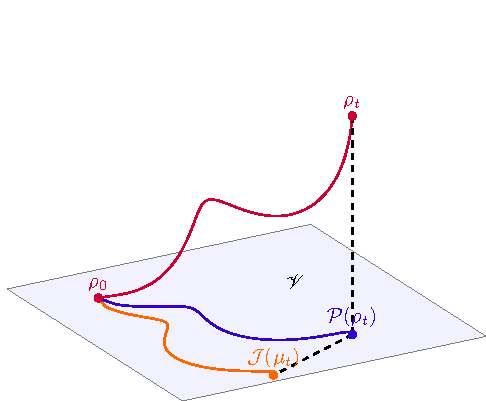
\includegraphics[width=\linewidth]{schematic.pdf}
    \caption{Graphical representation of the approximation problem. The pale blue plane represents the operator space $\Vs$ onto which $\Pc$ projects. The red curve represents the trajectory of the original model $\rho_t$, which starts in $\Vs$ at $t=0$.  The blue curve represents the projection of the true trajectory $\Pc(\rho_t)$, i.e. the one we want to approximate. Finally, the orange curve represents the approximate evolution we aim to find, i.e. $\Jc(\mu_t)$.}
    \label{fig:schematic}
\end{figure}

A graphical representation of the approximation problem is given in Fig.\,\ref{fig:schematic}.   

\subsection{Time-convolutionless master equation}

Before moving to the method proposed in this work for computing the time dependent generator $\Fc_t$ we shall discuss the derivation of time-convolutionless master equations, which is the standard method found in the literature \cite{Tokieda_2025, chaturvedi_time-convolutionless_1979, nestmann_time-convolutionless_2019, shibata_generalized_1977} to solve this issue . 

Dividing the evolution of $\rho_t$ in the evolution of $\Pc\rho_t$ and that of $\Qc\rho_t$ we have 
\begin{align*}
    \frac{d}{dt}\Pc \rho_t &= \Pc\Lc\Pc \rho_t + \Pc\Lc\Qc\rho_t,\\
    \frac{d}{dt}\Qc \rho_t &= \Qc\Lc\Pc \rho_t + \Qc\Lc\Qc\rho_t.
\end{align*}
Solving the second equation for $\Qc\rho_t$ we obtain
\[\Qc\rho_t = e^{\Qc\Lc\Qc t} \Qc\rho_0 + \int_0^t e^{\Qc \Lc \Qc s }\Qc \Lc \Pc \rho_{t-s} ds\]
and substituting this equation into the first equation we obtain the famous Nakajima-Zwanzig equation \cite{nakajima,zwanzig}:
\begin{align*}
    \frac{d}{dt}\Pc \rho_t = \Pc\Lc\Pc \rho_t &+ \Pc\Lc e^{\Qc\Lc\Qc t} \Qc\rho_0 \\&+\int_0^t \Pc\Lc\Qc e^{\Qc \Lc \Qc s }\Qc \Lc \Pc \rho_{t-s} ds.
\end{align*}
In order to derive the time-convolutionless master equation we recall that 
\(\rho_{t-s} = e^{-\Lc s}\rho_t\)
so that 
\[\Qc\rho_t = e^{\Qc\Lc\Qc t} \Qc\rho_0 +\int_0^t e^{\Qc \Lc \Qc s }\Qc \Lc \Pc e^{-\Lc s} ds\, \cdot\, (\Pc + \Qc) \rho_t. \]
Now, defining 
\[\Mc_t \equiv \Ic - \int_0^t e^{\Qc \Lc \Qc s }\Qc \Lc \Pc e^{-\Lc s} ds\]
we have 
\[\Mc_t \Qc\rho_t = e^{\Qc\Lc\Qc t} \Qc\rho_0 + (\Ic-\Mc_t) \Pc \rho_t\]
If we then assume that $\Mc_t$ is invertible for all $t\geq0$ we obtain 
\[\Qc\rho_t = \Mc_t^{-1}e^{\Qc\Lc\Qc t} \Qc\rho_0 + (\Mc_t^{-1} -\Ic) \Pc \rho_t\]
Substituting this inside the equation above we obtain 
\begin{align*}
    \frac{d}{dt}\Pc \rho_t &= \Pc\Lc\Pc \rho_t + \Pc\Lc \Mc_t^{-1}e^{\Qc\Lc\Qc t} \Qc\rho_0 \\& \qquad\qquad\qquad\qquad+ \Pc\Lc (\Mc_t^{-1}-\Ic) \Pc \rho_t\\ &= \Pc\Lc \Mc_t^{-1}e^{\Qc\Lc\Qc t} \Qc\rho_0 + \Pc\Lc \Mc_t^{-1} \Pc \rho_t.
\end{align*}
Note that under the assumptions that $\Pc\rho_0=\rho_0$ we have that $\Qc\rho_0=0$ and thus the equation gets simplified to 
\[\frac{d}{dt}\Pc \rho_t = \underbrace{\Pc\Lc \Mc_t^{-1} \Pc}_{\equiv\Kc_t} \rho_t\]
which gets simplified to 
\begin{equation}
    \frac{d}{dt}\eta_t = \underbrace{\Rc \Lc \Mc_t^{-1} \Jc}_{\equiv\Fc_t} \eta_t
\end{equation}
when separating the Projector $\Pc$ into its factors $\Rc = \Jc\Rc$.

Note that, in order to compute $\Fc_t$ (or equivalently $\Kc_t$) one needs to first compute the integral that defines $\Mc_t$ and then to compute the inverse of $\Mc_t$. Both these tasks are numerically challenging. 

To circumvent these numerical issues, $\Kc_t$ is typically approximated by expanding it as ordered cumulants \cite{breuer2002theory,breuer2006,nestmann2019time}:
\begin{align*}
    \Kc_t = \sum_{n=1}^\infty \Kc_n(t)
\end{align*}
where
\begin{align*}
    \Kc_n(t) &= \int_{0}^t dt_1 \int_0^{t_1} dt_2 \dots \int_0^{t_{n-2}}dt_{n-1}\\
    &\qquad \times \sum_q (-1)^q \Pc \Lc_{t} \dots \Lc_{t_i}\Pc\Lc_{t_j}\dots\Lc_{t_k}\Pc\dots\Pc
\end{align*}
where $\Lc_t$ is typically a time-dependent generator as the dynamics is often written in interaction picture. \TG{[Expand and study this better.]}

\TG{[Describe the drawbacks of this approach.]}



\section{Polynomial approximations of the time-dependent generator}

This work leverages a key assumption: I assume that the time dependent generator $\Fc_t$ is polynomial in $t$, i.e. $\Fc_{t,N} \equiv \sum_{k=0}^N t^k \Fc_{(k+1)}$. This assumption is clearly restrictive, but it greatly simplifies the computation of the time-ordered exponential $\Tb e^{\int_0^t \Fc_{s,N} ds}$ as shown in the next key result. 
\begin{theorem}
\label{thm:time_ordered_expansion}
    Let us assume that \(\Fc_{t,N} = \sum_{k=0}^{N} t^k \Fc_{(k+1)}\). 
    Then the time-ordered exponential can be written as
    \begin{equation}
        \Tb e^{\int_0^t \Fc_{s,N} ds} = \sum_{k=0}^{+\infty} t^k \Ec_{(k)}
        \label{eqn:time_ordered_expansion}
    \end{equation}
    where $\Ec_{(0)}=\Ic$ and 
    \begin{equation}
        \Ec_{(k)} =  \frac{1}{k} \sum_{s=1}^{k} \Fc_{(s)}\Ec_{(k-s)}
        \label{eqn:E_k}
    \end{equation}
    and where we used the convention $\Fc_{(k)}=0$ for all $k>N$.
\end{theorem}
Proof of this result and an explanatory example are given in Appendix \ref{sec:thechnical_results:time_ordered}.

Note that Eq. \eqref{eqn:E_k} provides a closed formula for the coefficients $\Ec_{(k)}$ of the expansion of $\Tb e^{\int_0^t \Fc_{s,N} ds}$ as a function of the coefficients $\Fc_{(k)}$. Furthermore, only the terms $\{\Ec_{(\ell)}\}_{\ell=1}^{k-1}$ appear in Eq. \eqref{eqn:E_k}, which means that this equation can be used iteratively to compute each term $\Ec_{(k)}$. 

Theorem \ref{thm:time_ordered_expansion} provides the main intuition on how to construct the polynomial time dependent generator $\Fc_{t,N}$: Eq. \eqref{eqn:time_ordered_expansion} provides an expansion for $\Tb e^{\int_0^t \Fc_{s,N} ds}$ in the time variable $t$. We can then expand $e^{t\Lc}$ in $t$ and construct $\Fc_{(k)}$ so that the terms of $\Tb e^{\int_0^t \Fc_{s,N} ds}$ match the terms of $\Rc e^{t\Lc} \Jc$ by orders of $t$, similarly to the procedure used in \cite{adiabadic-elimination}. 
The main result of this work, which summarizes the result of this procedure is stated next.
\begin{theorem}
\label{thm:approx}
Let us define 
\begin{equation}
\Fc_{t,N} \equiv \sum_{k=0}^{N} t^k \Fc_{(k+1)}
\label{eqn:poly_generator}
\end{equation}
where 
\begin{equation}
\Fc_{(k)} \equiv k\frac{\Rc \Lc^k \Jc}{k!} - \sum_{h=1}^{k-1}\Fc_{(k-h)}\frac{\Rc \Lc^h \Jc}{h!}.
\label{eqn:F_k}
\end{equation}
Then:
\begin{align}
\Rc e^{\Lc t}\Jc - \Tb e^{\int_0^t \Fc_{s,N} ds} = O(t^{N+1}).
\label{eqn:time_approx}
\end{align}
\end{theorem}
Before proceeding to prove this result we shall observe a few key aspects. First, it is important to notice that the right-hand side of equation \eqref{eqn:F_k} depends on $\Rc\Lc^{k}\Jc$ and $\{\Fc_{(s)}\}_{s=1}^{k-1}$. This means that equation \eqref{eqn:F_k} can be used iteratively to construct the terms $\Fc_{(k)}$ starting from $k=1$ and growing up to $k=N$. 
For the reader's convenience we write here the first few terms of the series:
\begin{align*}
    \Fc_{(1)} &= \Rc\Lc\Jc\\
    \Fc_{(2)} &= \Rc\Lc^2\Jc - \Fc_{(1)}\Rc\Lc\Jc = \Rc\Lc^2\Jc - (\Rc\Lc\Jc)^2\\
    \Fc_{(3)} &= \frac{\Rc\Lc^3\Jc}{2} - \Fc_{(2)}\Rc\Lc\Jc - \Fc_{(1)}\frac{\Rc\Lc^2\Jc}{2} \\
    &= \frac{\Rc\Lc^3\Jc}{2} - \frac{\Fc_{(1)}\Fc_{(2)}}{2} - \frac{\Fc_{(1)}^3}{2} - \Fc_{(2)}\Fc_{(1)}
\end{align*}
It is interesting to notice a couple of points about the first few terms: i) As one would expect, the term of order one $\Fc_{(1)}$ coincides with the reduction of the original dynamics which is often used as rough time-independent approximation of the reduced evolution \TG{[CITE]}; ii) The second order term does not only contain the reduction of the generator squared $\Rc\Lc^2\Jc$ but also contains a correction term depends on the first order term $\Fc_{(1)}$.  

Second, Eq. \eqref{eqn:time_approx} finally gives sense to the approximation symbol $\approx$ used in Sec. \ref{sec:problem_setting} i.e. an approximation of the type $O(t^{N+1})$. This implies that the approximation holds only for small times. 

We are finally ready to prove Theorem \ref{thm:approx}.
\begin{proof}
First of all we can use Theorem \ref{thm:time_ordered_expansion} to write 
\[\Tb e^{\int_0^t \Fc_{s,N} ds} = \sum_{f=0}^{+\infty} t^k \Ec_{(k)}\]
where \(\Ec_{(k)} =  \frac{1}{k} \sum_{s=1}^{k} \Fc_{(s)}\Ec_{(k-s)}= \frac{1}{k}\sum_{h=0}^{k-1} \Fc_{(k-h)}\Ec_{(h)}\) and where we reversed the order of the summation by imposing $h=k-s$. We next prove that, for $1\leq k \leq N$, we have $\Ec_{(k)}=\frac{\Rc\Lc^k\Jc}{k!}$ by induction. The case $k=1$ is trivial as $\Ec_{(1)} = \Fc_{(1)}\Ec_{(0)} = \Rc \Lc \Jc$. Let then assume that $\Ec_{(h)} = \frac{\Rc\Lc^h\Jc}{h!}$ for all $h<k$ and let us prove that $\Ec_{(k)}=\frac{\Rc \Lc^k \Jc}{k!}$. Then
\begin{align*}
    \Ec_{(k)} &= \frac{1}{k}\sum_{h=0}^{k-1} \Fc_{(k-h)}\Ec_{(h)} = \frac{\Fc_{(k)}}{k} + \frac{1}{k}\sum_{h=1}^{k-1}\Fc_{(k-h)}\Ec_{(h)}\\
    &= \frac{\Fc_{(k)}}{k} + \frac{1}{k}\sum_{h=1}^{k-1}\Fc_{(k-h)}\frac{\Rc \Lc^h \Jc}{h!}
    = \frac{\Rc \Lc^k \Jc}{k!}
\end{align*}
where we simply substituted the definition of $\Fc_{(k)}$ given in eq. \eqref{eqn:F_k}.

By leveraging the definition of the exponential map $e^{\Lc t}$ we can expand the term $\Rc e^{\Lc t}\Jc$ to obtain
\begin{align*}
    \Rc e^{\Lc t} \Jc = \sum_{k=0}^{+\infty} \frac{t^k}{k!} \Rc \Lc^k \Jc.
\end{align*}
Combining the two terms we obtain
\begin{align*}
    \Rc e^{\Lc t}\Jc - \Tb e^{\int_0^t \Fc_{s,N} ds} &= \sum_{k=0}^{+\infty}t^k\left(\frac{\Rc\Lc^k \Jc}{k!} - \Ec_{(k)}\right) \\
    &= \sum_{k=0}^{N}t^k\cancel{\left(\frac{\Rc\Lc^k \Jc}{k!} - \Ec_{(k)}\right)}\\ &\qquad\qquad + O(t^{N+1})
\end{align*}
which concludes the proof.
\end{proof}

\begin{remark}
    Note that in this section we have derived an approximation method that is applicable to any LTI system. In fact, in both Theorem \ref{thm:time_ordered_expansion} and Theorem \ref{thm:approx}, no assumption on the structure of $\Lc$ or $\Pc$ was used, implying that those results can be used to derive approximate models for ``classical'' linear systems as well, e.g. in cases where $\rho_t\in\Cb^n$, $\Lc,\Pc\in\Cb^{n\times n}$ and $\Fc_t\in\Cb^{m\times m}$ where $m=\dim{\rm Im}\Pc$.
    To showcase this point, in Sec. \ref{sec:linear_testbed} we study the problem of reducing a classical linear time-invariant model using the methods presented in this section.
\end{remark}

\subsection{Connection with the literature}

While the results I just presented have been derived independently, it shall be noted that a recursive formula similar to \eqref{eqn:F_k} have previously been proposed in the literature. Specifically \cite[Eq. (38)]{nestmann2019time} provides a recursive formula, similar to \eqref{eqn:F_k} for the terms of a Dyson expansion for the time-dependent generator $\Fc_t$. That formula however was derived starting from an initial time-dependent model and thus the terms of the recursive formula contain time-ordered integrals that need to be solved in order to compute the terms of the expansion. Because in this work I start from a time-independent model, Eq. \eqref{eqn:F_k} does not contain time-ordered integrals, resulting in overall simpler computations.

\TG{Other works in the literature have similar recursive formulas: Specifically, \cite[Eq. (2)]{cerrillo2014non} \cite[Eq. (2)]{cygorek2025timenonlocalversustimelocallongtime}, \cite[Eq. (16)]{gasbarri2018recursive}}

Another aspect that separates this work from most of the literature, e.g. \cite{colla2025unveiling,colla2025recursive,Tokieda_2025} is the fact that instead of expanding in a power-series of a perturbation parameter $\lambda$ or $\varepsilon$ that typically describes the coupling coefficient, here we expand in the time variable $t$. This fact simplifies the calculations and lifts the weak-coupling assumption that is typically introduced but comes at a cost: the approximate model holds only for small times.
This aspect however is not limiting as these reduced models are typically considered to hold only for small times. \TG{Argument better.}


\section{Complete Positivity of the approximate model at first and second order}

In this section we focus on the complete positivity of the reduced dynamics.

\subsection{First order}
\label{sec:cptp_first_order}

In this section we recall relevant known results about CPTP projectors, their images and reduced dynamics onto distorted algebras from the literature \cite{lindblad1999general, wolf2012quantum, ticozzi2017alternating, bialonczyk2018application, blume2010information,grigoletto2024exact,wolf2010inverseeigenvalueproblemquantum}. The consequences of the assumptions we made about the projector $\Pc$ are summarized in the following proposition. 
\begin{proposition}
\label{prop:structure_of_fixed_points}
    Let $\Pc$ be a CPTP projector with a full rank fixed point $\bar{\rho}>0$, $\Pc(\bar{\rho})=\bar{\rho}$ and let $\Vs$ be its image, i.e. $ \Vs \equiv {\rm Im}\Pc \subseteq\Bf(\Hc)$. 
    Then there exist a decomposition of the Hilbert space \[\Hc = \bigoplus_k (\Hc_{F,k}\otimes\Hc_{G,k}),\] a unitary operator $U\in\Bf(\Hc)$, and a set of density operators $\tau_k\in\Df(\Hc_{G,k})$ such that 
    \begin{equation}
        \Vs = U\left(\bigoplus_k \Bf(\Hc_{F,k}) \otimes \tau_k  \right) U^\dag.
        \label{eq:wedderburn_decomposition}
    \end{equation}
    Furthermore $\Vs$ is a $*$-algebra closed with respect to the product $X\cdot_\sigma Y \equiv X \sigma Y$ where \[\sigma = U\left(\bigoplus_k\one_{F,k}\otimes \tau_k^{-1}\right)U^\dag.\]  
    Let then $W_k$ be a linear operator from $\Hc$ onto $\Hc_{F,k}\otimes\Hc_{G,k}$ such that $W_k W_k^\dag=\one_{F,k}\otimes \one_{G,k}$ \cite{wolf2012quantum}. Then the CPTP projection $\Pc$ onto $\Vs$ takes the form
    \begin{align}
         \Pc(X) 
            &= U\left[ \bigoplus_{k} \tr_{\Hc_{G,k}}\left(W_k X W_k^\dag \right)\otimes \tau_k  \right] U^\dag.
        \label{eqn:state_ext_blocks}
    \end{align}
    and is orthogonal with respect to the inner produce $\inner{X}{Y}_{\sigma,\lambda} = \tr[X^\dag \sigma^\lambda Y \sigma^{1-\lambda}]$ for $\lambda\in[0,1]$.
\end{proposition}
Proof of this result can be found in \cite{lindblad1999general} and \cite{wolf2010inverseeigenvalueproblemquantum,wolf2012quantum,tit2023, ticozzi2017alternating, johnson2015general}. Note that projectors of this type take the name of state extensions and are the dual of conditional expectations \cite{petz2007quantum}. Furthermore, note that a $*$-algebra closed with respect to a modified product often takes the name of \textit{distorted algebra} \cite{blume2010information}, while the block structure provided in Eq.\,\eqref{eq:wedderburn_decomposition} takes the name of \textit{Wedderburn decomposition}. 

The previous result provides us with a structure for the image of a  CPTP projection whenever there exists a full rank state $\bar{\rho}$ such that $\Pc(\bar{\rho}) = \bar{\rho}$. From this structure one can observe that a distorted algebra $\Vs$ is isomorphic to a smaller representation which we denote $\As$ where the weighted copies are removed, i.e. $\As \equiv \bigoplus_k \Bf(\Hc_{F,k})$. This allows us to find the two factors $\Rc:\Bf(\Hc)\to{\As}$ and $\Jc:{\As}\to\Bf(\Hc)$ such that, $\Rc\Jc = \Ic_{{\As}}$ and $\Pc = \Jc\Rc$. 
Furthermore, one can observe \cite{grigoletto2024exact} that these two factors can be chosen to be CPTP, i.e. for all $X\in\Bf(\Hc)$
\begin{equation}
\label{eqn:reduction}
\Rc(X)=\bigoplus_k \tr_{\Hc_{G,k}}(W_k X W_k^\dag)=\bigoplus_k X_{F,k}=\check X ,
\end{equation}
and for all $\check{X}\in\check{\As}$, $\check{X}=\bigoplus_k X_{F,k}$,
\begin{equation}
\label{eqn:injection}
\es(\check X)=U\bigg(\bigoplus_k X_{F,k} \otimes\tau_{k}\bigg)U^\dag.
\end{equation}

The reduction and injection maps given in equations \eqref{eqn:reduction} and \eqref{eqn:injection} then allow to compute the reduced dynamics $ \Rc\Lc\Jc$ restricted onto the algebra ${\As}$. One can then prove that the reduced generator $\check{\Lc}$ is GKLS by leveraging the structure of the reduction and injection maps. We here report \cite[Theorem 4]{grigoletto2024exact} for completeness.
\begin{theorem}
\label{thm:Lindblad_reduction}
Let $\Pc$ be a CPTP projection with a full rank fixed point, let $\mathscr{V}$ be its image $\Vs = {\rm Im }\Pc \subseteq \mathcal{B(H)}$, and let $\Rc$ and $\Jc$ denote the CPTP factorization of $\Pc = \Jc\Rc$, as defined in Eq.\,\eqref{eqn:reduction} and \eqref{eqn:injection}. Then for any Lindblad generator $\Lc$, its restriction to ${\As}$, 
$\Rc\Lc\Jc,$ 
is also a Lindblad generator, that is, $\Rc\Lc\Jc:\As\to\As$ and $\{e^{\check{\Lc}t}\}_{t\geq 0}$ is a quantum dynamical semi-group. 
\end{theorem}
Note that this theorem only proves the fact that $\Rc\Lc\Jc$ is of Lindblad type. In order to compute the reduced Hamiltonian and noise operators one can use the procedure described in \cite[Appendix]{grigoletto2025quantummodelreductioncontinuoustime}.


\subsection{Second order: The case of purely Hamiltonian evolution}

While the results we derived up to this point hold for general Lindblad generators $\Lc$, we shall now focus on the special case of purely Hamiltonian evolution, i.e. $\Lc(\cdot) = -i[H,\cdot].$ Other than the fact that this assumption is interesting in practical cases, we shall see that under this simplifying assumption we are able to prove that the second order term $\Fc_{(2)}$ is also of Lindblad-type.

The next result is based on the fact that the squared of a purely Hamiltonian generator is equal to a dissipator:
\begin{align}
    \Lc^2(\rho) &= - [H[H,\rho]] = -(H^2\rho - 2H\rho H + \rho H^2)\nonumber \\
    &= 2H\rho H - \{H^2,\rho\} = \Dc_{\sqrt{2}H}(\rho).
    \label{eqn:square_hamiltonian}
\end{align}
This fact allows us to prove the next result.
\begin{theorem}
\label{thm:cptp_second_order}
    Under the assumptions of Theorem \ref{thm:Lindblad_reduction} we have that $\Fc_{(2)} = \Rc\Lc^2\Jc - (\Rc \Lc \Jc)^2$ is of Lindblad-type and for $\Fc_{t,2} \equiv \Fc_{(1)} + t \Fc_{(2)}$ we have that $\Tb e^{\int_0^t \Fc_{s,2} ds}$ forms a set of CPTP maps for all $t\geq0$. 
\end{theorem}
\begin{proof}
    By leveraging \cite[Proposition 5]{grigoletto2024exact} we have that $\Rc\Lc\Jc(\check{\rho}) = -i[\check{H},\check{\rho}]$ where $\check{H} = \Jc^\dag(H)$ hence, using equation \eqref{eqn:square_hamiltonian} we obtain $(\Rc\Lc\Jc)^2(\check{\rho}) = \Dc_{\sqrt{2}\check{H}}(\check{\rho})$. On the other hand, by leveraging \cite[Proposition 6 and Proposition 7]{grigoletto2025quantummodelreductioncontinuoustime}, we have that $\Rc \Dc_{\sqrt{2}H}\Jc(\check{\rho}) = \sum_{\check{C}\in\Xc(\sqrt{2}H)} \Dc_{\check{C}}(\check{\rho})$ for a set of operators $\Xc(\sqrt{2}H)\subset \Bf(\Kc)$. Importantly, by \cite[Corollary 4]{grigoletto2025quantummodelreductioncontinuoustime}, we have that $\Jc^\dag(H)\in\Xc(\sqrt{2}H)$ and thus we can write $\Rc \Dc_{\sqrt{2}H}\Jc(\check{\rho}) = \sum_{\check{C}\in\Xc(\sqrt{2}H)/\{\sqrt{2}\check{H}\}} \Dc_{\check{C}}(\check{\rho}) + \Dc_{\sqrt{2}\check{H}}(\check{\rho})$ since $\sqrt{2}\check{H} = \Jc^\dag(\sqrt{2}H)$. Then, by combining these two results we obtain 
    \[ \Fc_{(2)} = \Rc\Lc^2\Jc - (\Rc \Lc \Jc)^2 = \sum_{\check{C}\in\Xc(\sqrt{2}H)/\{\sqrt{2}\check{H}\}} \Dc_{\check{C}}(\check{\rho}) \]
    which is the sum of a set of GKLS, purely dissipative generators and thus of Lindblad type. Combining this with Theorem \ref{thm:Lindblad_reduction} it trivially follows that $\Fc_{t,2}$ is of Lindblad type for all $t\geq0$.
\end{proof}
\subsection{Second order in the special case of bipartite systems}
\label{sec:second_order_bipartite}
Because the proof of Theorem \ref{thm:cptp_second_order} is based on a few very technical results, we here want to present an equivalent pedagogical derivation of the same result. Note that this derivation is quite relevant in practice as it focuses on the most studied case of a bi-partite system but the cases included in the assumptions of Theorem \ref{thm:cptp_second_order} are more general. This exact case will be the focus of the two applications of interest studied in Sec \ref{sec:spin_boson} and \ref{sec:central_spin}.

Let us assume that $\Hc = \Hc_S\otimes\Hc_E$ and let assume that the CPTP projector $\Pc$ is given by the $\Pc(\cdot) = \tr_E(\cdot)\otimes\tau$ for some full rank state $\tau\in\Df(\Hc_E)$. The projector $\Pc$ is then factorized into the reduction map $\Rc(\cdot) = \tr_E(\cdot)$ and the injection map $\Jc(\cdot) = \cdot\otimes \tau$. 
In line with the assumptions of this section we assume that $\Lc(\cdot) = -i \ad_H(\cdot)$. Given the bipartite structure of the Hilbert space $\Hc$ we can always write $H = \sum_k S_k \otimes E_k$ for two sets of Hermitian operators $\{S_k\}\subset\Bf(\Hc_S)$ and $\{E_k\}\subset\Bf(\Hc_E)$.

We can then proceed to compute the reduced generator approximated at second order $\Fc_{t,2}(\mu)$. First, using \cite[Proposition 5]{grigoletto2024exact}, we have that the generator at first order is \[\Fc_{(1)}(\mu) = \Rc \Lc \Jc(\mu) = -i[\check{H},\mu]\] where
\begin{align*}
    \check{H} &= \Jc^\dag(H) = \tr_{E}[(\one_S\otimes\tau) H] %= \sum_k \tr_E[S_k \otimes (\tau E_k)]\\ &
    = \sum_k a_k(\tau) S_k
\end{align*}
and $a_k(\tau) \equiv \tr[\tau E_k]. $ Next, we can proceed to compute $\Fc_{(2)}$ by first computing $\Rc \Lc^2 \Jc$:
\begin{widetext}
    \begin{align*}
    \Rc \Lc^2 \Jc(\mu) &= \sum_{j,k} \tr_E[ 2(S_j\otimes E_j) (\mu\otimes\tau) (S_k\otimes E_k) - (S_k\otimes E_k)(S_j\otimes E_j) (\mu\otimes\tau)  - (\mu\otimes\tau) (S_k\otimes E_k) (S_j\otimes E_j) ] \\
    &= \sum_{j,k} 2 S_j \mu S_k \underbrace{\tr[ E_j\tau E_k]}_{\equiv c_{j,k}(\tau)} - S_kS_j \mu \underbrace{\tr[E_kE_j\tau]}_{=c_{j,k}(\tau)} - \mu S_kS_j \underbrace{\tr[\tau E_kE_j ]}_{=c_{j,k}(\tau)} \\
    &= \sum_{j,k} c_{j,k}(\tau) \left[2S_j \mu S_k - \{ S_kS_j, \mu\}  \right].
\end{align*}
\end{widetext}
On the other hand, since $(\Rc\Lc\Jc)^2 = \Dc_{\sqrt{2}\check{H}}$, we have
\begin{align*}
    (\Rc\Lc\Jc)^2(\mu) = \sum_{j,k}  a_j(\tau)a_k(\tau) \left[ 2 S_j \mu S_k - \{S_kS_j,\mu\} \right]
\end{align*}
and thus 
\begin{align*}
    \Fc_{(2)}(\mu)&=[\Rc \Lc^2 \Jc  - (\Rc\Lc\Jc)^2](\mu) =\\ &=\sum_{j,k} [\chi(\tau)]_{j,k} \left[2S_j \mu S_k -  \{ S_kS_j, \mu\}  \right]
\end{align*}
where we defined the matrix $\chi(\tau)$ whose elements are $[\chi(\tau)]_{j,k} \equiv c_{j,k}(\tau)-a_j(\tau)a_k(\tau)$.
One can then notice that the matrix $\chi(\tau)$ coincides with a covariance matrix, i.e. 
\begin{align*}
    [\chi(\tau)]_{j,k} &= \tr[E_j \tau E_k] - \tr[E_j\tau]\tr[E_k\tau]\\
    &= \Eb_\tau[(E_k - \Eb_\tau[E_k]\one_E) (E_j - \Eb_\tau[E_j]\one_E)]
\end{align*}
hence $\chi(\tau)$ is a positive semi-definite matrix.
Since $\chi(\tau)$ is positive semi-definite, it is diagonalizable with a unitary matrix, i.e. $UU^\dag =U^\dag U = \one$ such that $U\chi(\tau) U^\dag = \gamma(\tau)$ where $\gamma(\tau)$ is a diagonal matrix of positive values (note that in reality $U$ is also a function of $\tau$). We can then define 
\[L_h = \sum_j \overline{[U]_{h,j}} S_j \]
to obtain 
\begin{align*}
\Fc_{(2)}(\mu) 
&=\sum_{j,k} [\chi(\tau)]_{j,k} \left[2S_j \mu S_k - \{ S_kS_j, \mu\}  \right]\\
&=\sum_{j,k,h} \underbrace{[U^\dag]_{j,h}[\gamma(\tau)]_{h} [U]_{h,k}}_{[\chi(\tau)]_{j,k}} \left[2 S_j \mu S_k - \{ S_k S_j, \mu\}  \right]\\
&=\sum_{j,k,h} [\gamma(\tau)]_{h} \overline{[U]_{h,j}}[U]_{h,k} \left[2 S_j \mu S_k - \{ S_k S_j, \mu\}  \right]\\
&=\sum_h [\gamma(\tau)]_{h} \left[2L_h \mu L_h^\dag - \{ L_h^\dag L_h, \mu\}  \right] \\
& = \sum_h [\gamma(\tau)]_h \Dc_{\sqrt{2} L_h}(\mu).
\end{align*}
Because $\chi(\tau)$ is positive-semidefinite and thus $[\gamma(\tau)]_h$ are non-negative, then $\Fc_{(2)}$ is of Lindblad type. This implies that the approximated time-dependent generator approximated at second order 
\[\Fc_{t,2}(\mu) = -i[\check{H},\mu] + \sum_h t [\gamma(\tau)]_h \Dc_{\sqrt{2} L_h}(\mu)\]
is also of Lindblad type at all times $t\geq0$ as proved in Theorem \ref{thm:cptp_second_order}.

Note that in deriving the reduced generator $\Fc_{t,2}$ there was no need to move the system's description into rotating frame. This provides another benefit of the proposed approach. 

\begin{figure*}[th]
    \centering
    \begin{subfigure}{0.48\textwidth}
        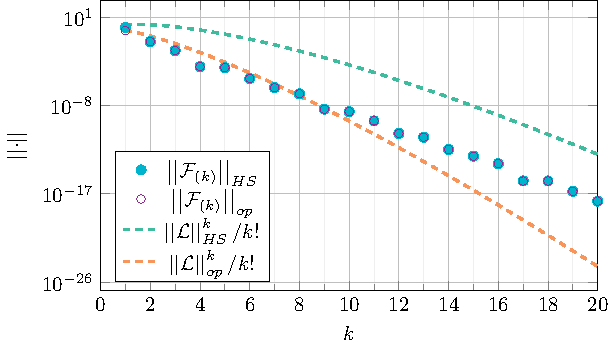
\includegraphics[width=\linewidth]{norm_bound.pdf}
    \end{subfigure}
    \begin{subfigure}{0.48\textwidth}
        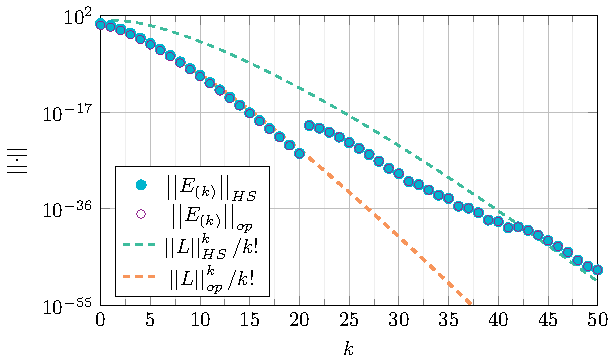
\includegraphics[width=\linewidth]{E_norm_bound.pdf}
    \end{subfigure}
    \caption{Operator and Hilbert-Schmidt norm of the first 20 $\Fc_{(k)}$ terms (left) and of the first 50 $\Ec_{(k)}$ terms when with $N=20$ (right).}
    \label{fig:norm_bound}
\end{figure*}

\section{Applications of interest}
\label{sec:applications}

The code necessary to reproduce the numerical experiment is available at \cite{Myrepo}.

\subsection{Linear testbed}
\label{sec:linear_testbed}

To showcase the capability of the method we here consider a simple numerical example.  
Specifically, we consider a random autonomous and stable system of size $n=20$. 
Let then $\Ac$ be a random uniform matrix in $\Cb^{n\times n}$, i.e. $[\Ac]_{i,j}\sim\Uc([0,1])$ and let $\Bc = \Ac - \lambda_{\rm Max} \one_{n\times n}$ where $\lambda_{\rm Max}$ is the absolute value of largest eigenvalue of $\Ac$. 
The dynamic's generator $\Lc\in\Cb^{n\times n}$ is then obtained as $\Lc = \frac{1}{2}\frac{\Bc}{\norm{\Bc}_{op}}$ where $\norm{\cdot}_{op}$ denotes the operator norm.
This ensures that $\Lc$ is simply stable and has operator norm $\norm{\Lc}_{op}=\um$. 

The projector $\Pc$ is then constructed through $\Rc = \left[\begin{array}{c|c} \one_{m\times m} & 0_{m\times n-m} \end{array}\right]$ and $\Jc = \Rc^\dag$ to obtain \[\Pc = \left[\begin{array}{c|c} \one_{m\times m} & 0_{m\times n-m} \\\hline 0_{m \times n-m } & 0_{n-m\times n-m} \end{array}\right].\]

By using Eq. \eqref{eqn:F_k} we can then compute the terms $\Fc_{(k)}$ iteratively for $k=1,\dots,N$. Fig. \ref{fig:norm_bound} (left) shows both the Hilbert-Schmidt and operator norm of the terms $\Fc_{(k)}$ for $k=1,20$. Interestingly, the Hilbert-Schmidt norm, $\norm{\Fc_{(k)}}_{HS}$, is bounded by $\frac{\norm{\Lc}_{HS}^k}{k!}$, indicating that the series $\Fc_{t,N}$ should be converging for $N\to\infty$. \TG{Curiously, the same does not hold for the operator norm.}
Fig. \ref{fig:norm_bound} (right) instead shows the norm of the terms $\Ec_{(k)}$ where we fixed $N=20$ and $\Fc_{(k)}=0$ $\forall k>20$. Interestingly for $k\leq N$ $\norm{\Ec_{(k)}}$ is bounded by $\frac{\norm{\Lc}^k}{k!}$ while for $k>N$ this is no longer the case.  

\begin{figure}[th]
    \centering
    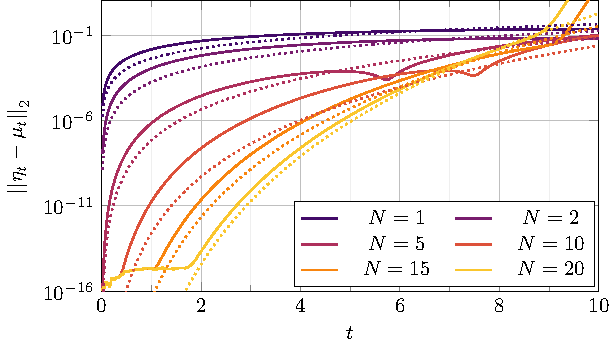
\includegraphics[width=\linewidth]{error_linear.pdf}
    \caption{Error norm between the exact reduced evolution $\eta_t$ and the approximated reduced evolution $\mu_t$ for different values of the approximation order $N$. The dotted curves represent a curve-fit for the function $\alpha t^{N+1}$ for different values of $N$. }
    \label{fig:error_linear}
\end{figure}

Fig. \ref{fig:error_linear} shows the error norm $\norm{\eta_t-\mu_t}_2$ versus time. In this simulation $\eta_t$ was simulated by reducing the original model, i.e. $\eta_t= \Rc e^{\Lc t}\rho_0$ while $\mu_t$ is obtained by simulating the time-dependent linear differential equation $\dot{\mu}_t=\Fc_{t,N}\mu_t$, for different values of $N$, by using an approximation of the equation given in Theorem \ref{thm:time_ordered_expansion}, i.e. \(\Tb e^{\int_0^t \Fc_{s,N} ds} \approx \sum_{k=0}^{100} t^k \Ec_{(k)}\).  
One can note that increasing the degree of approximation $N$ decreases the error committed by the approximated model. %Furthermore, by the curve-fit we can note that the error evolves approximately with $t^{N}$ indicating that the error indeed scales as $O(t^{N+1})$ as stated in Theorem \ref{thm:approx}.  

\subsection{Dephasing spin boson model}
\label{sec:spin_boson}



Inspired by \cite{lidar2001completely, reina2002decoherence, breuer2002theory, lidar2020lecturenotestheoryopen}, in this section we consider a dephasing spin-boson model to further showcase the advances and drawbacks of the proposed method. Note that: i) in this section we make an exception to the assumption of final dimensional systems considered throughout the paper; ii) the model I am going to consider is exactly solvable hence the intent of this subsection is to showcase that the proposed approximation method provides results comparable to other approximation techniques, not to compare it against the exact solution of the model. 
Nevertheless, this example helps us to understand the degrees of approximation that the proposed method offers and how the process unfolds.

The model is composed of a spin $\um$ system $\Hc_S\simeq\Cb^2$ coupled to a bath $\Hc_B$ composed of $N_B$ bosonic modes, $\Hc = \Hc_S\otimes \Hc_B$.The model's dynamcis is driven by the total Hamiltonian $H= H_S\otimes \one_B + \one_S \otimes H_B + H_{\rm int}$ where 
\begin{align}
    H_S &= \frac{g}{2}\sigma_z\\
    H_B &= \sum_{k=1}^{N_B} \omega_k \left(n_k+\frac{\one}{2}\right)\\
    H_{\rm int} &= \sigma_z \otimes \left(\sum_{k=1}^{N_B}\lambda_k b_k + \overline{\lambda}_k b_k^\dag\right)
\end{align} 
and where $n_k = b_k^\dag b_k$ and $b_k$ are the bosonic number and annihilation operator for mode $k$ respectively and satisfy $[b_k,b_l^\dag]=\delta_{k,l}\one$, $\omega_k\in\Rb$ is the mode frequency and $\lambda_k\in\Cb$ is the strength of the coupling between the mode and the spin.  

We assume the initial state to be factorized $\rho_0 = \rho_{S,0}\otimes\rho_B$ with $\rho_B = e^{-\beta H_B}/\tr[e^{-\beta H_B}]$ and some state $\rho_{S,0}\in\Df(\Hc_S)$ for the spin. We further assume the projector $\Pc$ to be $\Pc(\rho) = \tr_B(\rho)\otimes \rho_B$ which can be factorized into $\Rc(\rho) = \tr_B(\rho)$ and $\Jc(\sigma)=\sigma\otimes\rho_B$. One can then verify that $\Pc(\rho_0) = \rho_0$ and thus Assumption \ref{ass:proj} is satisfied. 

This model has a known exact analytical solutions given by \cite[eq. (336) and (374)]{lidar2020lecturenotestheoryopen}:
\[\rho_{S,t}' = \begin{bmatrix}
[\rho_{S,0}]_{0,0}&e^{-2\gamma(t)t}[\rho_{S,0}]_{0,1}\\
e^{-2{\gamma(t)}t}[\rho_{S,0}]_{1,0}&[\rho_{S,0}]_{1,1}\\
\end{bmatrix}\]
where $\rho_{S,t}'$ is the spin's state in the rotating frame and  
\(\gamma(t) = \sum_k \alpha_k \frac{1-\cos(\omega_k t)}{t}\)
with $\alpha_k \equiv 2\frac{|\lambda_k|^2}{\omega_k^2}\coth\left(\frac{\beta\omega_k}{2}\right)\in\Rb.$
By taking the derivative of an off diagonal element we obtain:
\[\frac{d}{dt}[{\rho}_{S,t}']_{0,1} = -2\underbrace{\left[\gamma(t) + \frac{d\gamma(t)}{dt}t\right]}_{\equiv \xi(t)}[{\rho}_{S,t}']_{0,1}\]
where \(\xi(t) = \sum_k\alpha_k\omega_k\sin(\omega_k t)\).
This dynamics corresponds to the differential equation 
\( \frac{d}{dt}\rho_{S,t}' = \xi(t)\Dc_{\sigma_z}[\rho_{S,t}']\)
for the state in rotating frame or, equivalently, to
\begin{equation}
    \dot{\rho}_{S,t} = -i[H_S,\rho_{S,t}] + \xi(t) \Dc_{\sigma_z}(\rho_{S,t})
    \label{eq:exact_boson}
\end{equation} 
for the state in the lab frame. 

By following the procedure detailed in Sec. \ref{sec:second_order_bipartite} we can then proceed to compute the reduced time-dependent generator at second order $\Fc_{t,2}$. 
Denoting $\expect{X}_B \equiv \tr[\rho_B X]$, we recall that \cite[eq. (331)]{lidar2020lecturenotestheoryopen}: 
\begin{align*}
    \expect{b_k^\dag}_B &= \expect{b_k}_B = \expect{b_k^\dag b_l^\dag}_B = \expect{b_k b_l}_B = 0,\\
    \expect{b_j^\dag b_k}_B &= \frac{\delta_{j,k}}{e^{\beta\omega_k}-1}.
\end{align*}
We first compute the reduced Hamiltonian $\check{H} = \Jc^\dag(H)$ where $\Jc^\dag(X) = \tr_B[X(\one_S\otimes\rho_B)]$. By noting that $\tr_B[H_S\otimes\one_B(\one_S\otimes\rho_B)] = H_S \tr[\rho_B] = H_S$, $\tr_B[\one_S\otimes H_B(\one_S\otimes\rho_B)] = \one_S \expect{H_B}_B$ and
\begin{align*}
    &\tr_B\left[\sigma_z\otimes\left(\sum_{k=1}^{N_B}\lambda_k b_k + \overline{\lambda}_k b_k^\dag\right)(\one_S\otimes\rho_B)\right]\\ &\qquad = \sigma_z \left( \sum_{k=1}^{N_B}\lambda_k \cancel{\expect{b_k}_B} + \overline{\lambda}_k \cancel{\expect{b_k^\dag}_B} \right) = 0
\end{align*}
we have \(\check{H} = H_S \) as the term \(\one \expect{H_B}_B\) only contributes to a phase and can thus be removed leading to the first order term $\Fc_{(1)}(\mu) = -i[\check{H},\mu]$. The second order term is instead found to be $Fc_{(2)}(\mu) = \varphi \Dc_{\sigma_z}(\mu)$ with $\varphi\equiv \sum_{k=1}^{N_B} \frac{2|\lambda_k|^2}{e^{\beta \omega_k}-1}$. All the necessary calculations are detalied in Appendix \ref{sec:spin_boson_model_calculations} for the sake of clarity. 

Combining both terms we obtain an approximate reduced model descibed by the time-dependent Lindblad equation
\begin{equation}
    \dot{\mu}_t = -i[H_S,\mu_t] + \varphi t \Dc_{\sigma_z}(\mu_t).
    \label{eq:time_ordered_boson}
\end{equation} 
By comparing this equation with the exact solution of Eq. \eqref{eq:exact_boson} we can observe that both the Hamiltonian and noise operator are correctly recovered whereas the time-dependent dissipation strength $\xi(t)$ is approximated with $\varphi t$. Interestingly, the value $\varphi$ does not coincide with the first order Taylor expansion of $\xi(t)$ which is $\sum_k\alpha_k\omega_k$.

\begin{figure*}
    \centering
    \begin{subfigure}{0.48\textwidth}
        \centering
        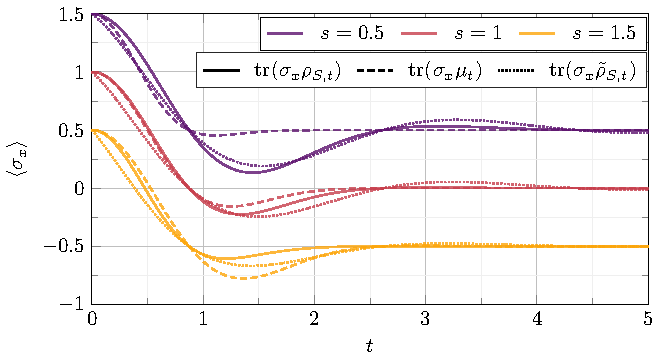
\includegraphics[width=\linewidth]{trajectory_spin_boson.pdf}
    \end{subfigure}
    \begin{subfigure}{0.48\textwidth}
        \centering
        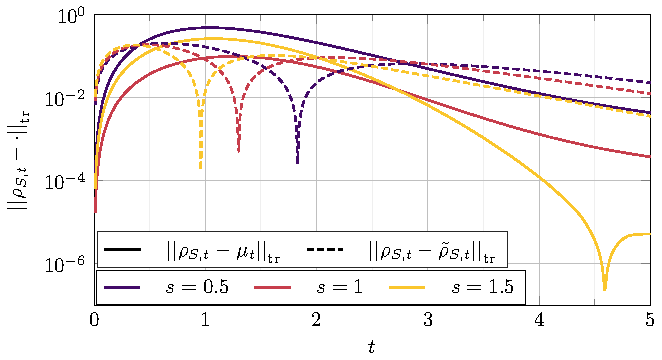
\includegraphics[width=\linewidth]{error_spin_boson.pdf}
    \end{subfigure}
    \caption{Simulation of the dephasing spin-boson model for $s=0.5,1,1.5$ where we compare the exact solution $\rho_{S,t}$ given in Eq.\eqref{eq:exact_boson}, the second order approximation $\mu_t$ derived in this work, given in Eq. \eqref{eq:time_ordered_boson} and the coarse-grained dynamics $\tilde{\rho}_{S,t}$ given in Eq. \eqref{eq:coarse_grained_boson}. Left: Evolution of the expectation value $\expect{\sigma_x}$ for the exact solution (continuous curves), second order approximation (dashed curve) and coarse-grained dynamics (dotted curve). The expectations values of the cases $s=0.5,1.5$ have been shifted by $\pm0.5$ respectively for graphical purposes. Right: evolution of the trace-norm error with respect to the exact solution committed by the second order approximation (continuous curve) and coarse-grained dynamics (dashed curve).   }
    \label{fig:dephasing_spin_boson}
\end{figure*}

To better asses the quality of the reduced second order approximation we next compare the evolution of $\rho_{S,t}$ and that of $\mu_t$ with the coarse-grained approximation discussed in \cite[eq. (332)]{lidar2020lecturenotestheoryopen}, i.e. \(\tilde{\rho}_{S,t}\in\Df(\Hc_S)\) and
\begin{equation}
    \dot{\tilde{\rho}}_{S,t} = -i[H_S,\tilde{\rho}_{S,t}] + \gamma(\tau)\Dc_{\sigma_s}(\tilde{\rho}_{S,t})
    \label{eq:coarse_grained_boson}
\end{equation}
where the constant $\tau\in\Rb$ is specified later. 

The bath coupling coefficients are going to be defined as $\lambda_k = \sqrt{J(\omega_k)}$ \cite{tamascelli2020quantum} where $J(\omega)$ is the bath spectral density and is chosen to be 
\begin{equation}
    J(\omega) = \Lambda \omega_c^{1-s} \omega^s e^{-\frac{\omega}{\omega_c}}
\end{equation}
where $\Lambda\in\Rb_+$ is an overall constant, $\omega_c\in\Rb_+$ is the bath cutoff frequency and $s\in\Rb_+$ is the Ohmicity parameter which determines three cases of interest, i.e. Ohmic ($s=1$), sub-Ohmic($s<1$) and super-Ohmic ($s>1$) \cite{PhysRevB.92.195143}.

In Fig. \ref{fig:dephasing_spin_boson} the results of the simulations are shown in the three cases, i.e. $s=0.5,1,1.5$. The other parameters used in the simulations are $g=1.8$, $\omega_c =0.2$, $\Lambda=0.5$, $\beta=10$, $\tau=32/\omega_c$, and where $\omega_k$ are $N_B=100$, taken equally spaced between $0$ and $1$. The initial state instead has been fixed to $\rho_{S,0}=\mu_0 = \tilde{\rho}_{S,0} = \ketbra{+}{+}$. 
Importantly, one can observe in Fig. \ref{fig:dephasing_spin_boson} Right that, in each of the three cases, the error committed by the second order approximation, Eq. \eqref{eq:time_ordered_boson} is below that of the coarse-grained dynamics, Eq. \eqref{eq:coarse_grained_boson} for both the initial and final phases while it is above for a central phase.     

\TG{This indicates that the second order approximation performs better than the coarse-grained Markovian approximation in this case.}

\subsection{Highly non-Markovian model}
\TG{\cite{breuer2006,breuer2007,gemmer2005thermalization, Riera2021}}

\subsection{Dissipative central spin model}
\label{sec:central_spin}

% \begin{figure}[th]
%     \centering
%     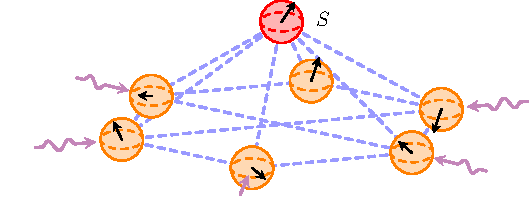
\includegraphics[width=.8\linewidth]{central_spin_figure.pdf}
%     \caption{Graphical representation of the dissipative central spin model.}
%     \label{fig:central_spin_figure}
% \end{figure}

\begin{figure*}
    \centering
    \begin{subfigure}{0.48\textwidth}
        \centering
        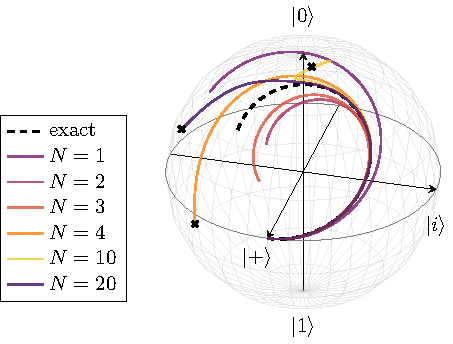
\includegraphics[width=.8\linewidth]{central_spin_bloch.pdf}
    \end{subfigure}
    \begin{subfigure}{0.48\textwidth}
        \centering
        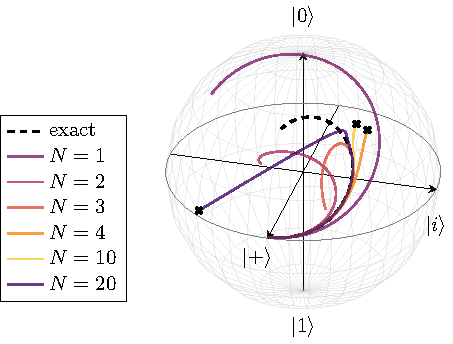
\includegraphics[width=.8\linewidth]{dissipative_central_spin_bloch.pdf}
    \end{subfigure}
    \begin{subfigure}{0.48\textwidth}
        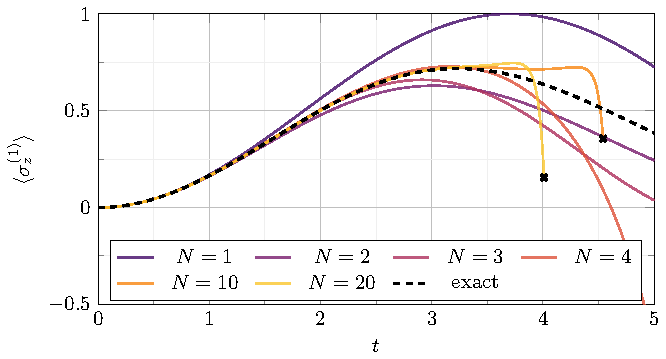
\includegraphics[width=\linewidth]{trajectory_central_spin.pdf}
    \end{subfigure}
    \begin{subfigure}{0.48\textwidth}
        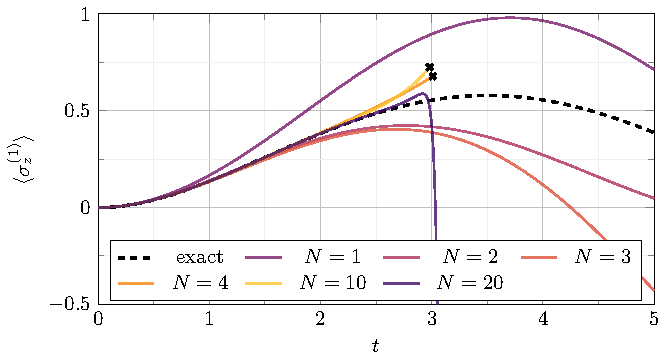
\includegraphics[width=\linewidth]{trajectory_dissipative_central_spin.pdf}
    \end{subfigure}
    \begin{subfigure}{0.48\textwidth}
        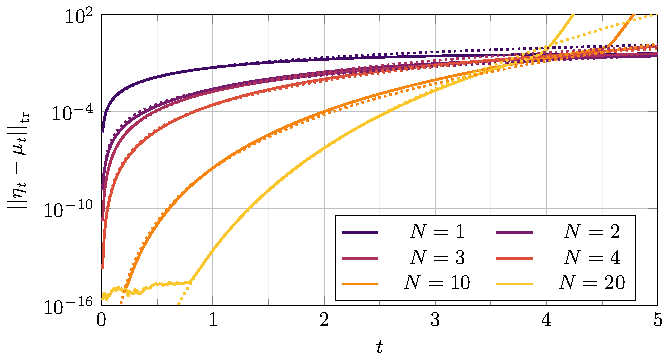
\includegraphics[width=\linewidth]{error_central_spin.pdf}
    \end{subfigure}
    \begin{subfigure}{0.48\textwidth}
        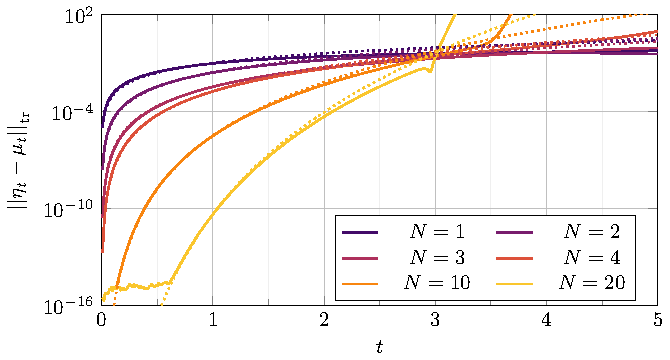
\includegraphics[width=\linewidth]{error_dissipative_central_spin.pdf}
    \end{subfigure}
    \caption{Simulations of the dissipative central spin model in the purely Hamiltonian setting (\(\Lambda=0\)) on the left and in the dissipative setting (\(\Lambda=0.8\)) on the right. The exact evolution and various degrees of approximations (\(N=1,2,3,4,10,20\)) are shown in each figure. The first row shows the trajectory of the central spin's state \(\rho_S\) in the Bloch sphere; the second row shows the magnetization of the central spin in the $\sigma_z$ direction versus time; the third row shows the trace norm error between the exact trajectory $\eta_t$ and the reduced one $\mu_t$, i.e. $\norm{\eta_t-\mu_t}_{\tr}$ versus time for different values of the approximation $N$ and with dotted curve representing a fitted $\alpha t^{N+1}$ curve.  The black crosses denote points where the evolved state $\mu_t$ exits the set of density operators.  }
    \label{fig:central_spin}
\end{figure*}




In this section we consider a dissipative central spin model to showcase the capabilities of the proposed technique. Similar models have been studied in the literature, see e.g. \cite{barnes2012nonperturbative, tiwari2025strong, jing2018decoherence, ferraro2008}. The model is composed by a system, i.e. $\Hc_S\simeq\Cb^2$ also denoted as spin $1$ and a bath composed of $N_B$ other spins, i.e. $\Hc_B\simeq\Cb^{2^{N_B}}$ counted from $2$ to $N_B+1$. %A graphical representation of the system is depicted in Fig.\ref{fig:central_spin_figure}.

The system Hamiltonian is described as $H = H_S + H_B + H_{\rm int}$ where:
\begin{align*}
    H_S &= \delta(\sigma_x^{(1)} + \sigma_z^{(1)})\\
    H_B &= \frac{\gamma}{4}\left(2J_x^2-\frac{N_B}{2}\one\right)\\
    H_{\rm int} &= \frac{\lambda}{2}\left(A_x \sigma_x^{(1)}J_x+ A_y \sigma_y^{(1)}J_y+A_z \sigma_z^{(1)}J_z\right)
\end{align*}
where $\sigma_u^{(j)}$ denotes the $u\in\{x,y,z\}$ Pauli matrix acting on the $j$-th spin and $J_u=\frac{1}{2}\sum_{k=2}^{N_B+1}\sigma_u^{(k)}$ denotes the total bath angular momentum operators. The bath is also in contact with a Markovian environment that dissiapates information. This interaction is described by the noise operators $L_k = \Lambda\sigma_-^{(k)}$ for all $k=2,\dots,N_B+1$ where $\sigma_\pm^{(k)} = \frac{1}{2}(\sigma_x^{(k)}\pm\sigma_y^{(k)})$.


\begin{figure*}[th]
    \centering
    \begin{subfigure}{0.49\textwidth}
        \centering
        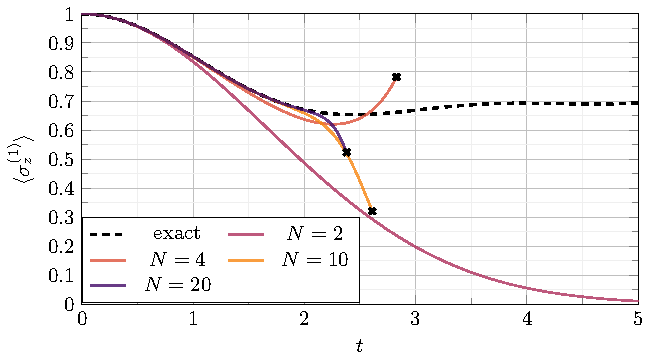
\includegraphics[width=\linewidth]{trajectory_spin_chain.pdf}
    \end{subfigure}
    \begin{subfigure}{0.49\textwidth}
        \centering
        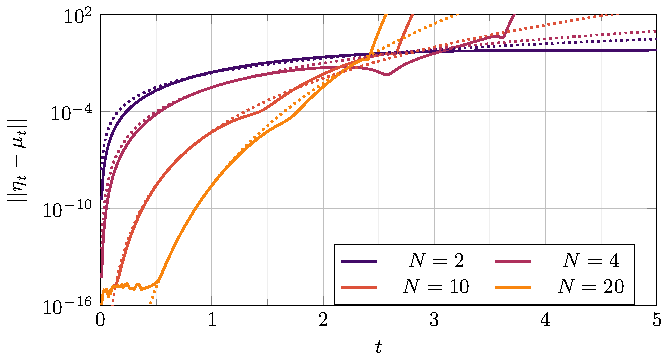
\includegraphics[width=\linewidth]{error_spin_chain.pdf}
    \end{subfigure}
    \caption{Simulation of the Ising spin chain. Magnetization of the first spin of the chain $\expect{\sigma_z^{(1)}}$ versus time on the left and the error norm $\norm{\eta_t-\mu_t}_2$ versus time on the right. Various approximation's degrees $N=2,4,10,20$ are shown in each figure. The black crosses denothe points where the evolved state $\mu_t$ exits the $n$-dimensional simplex, i.e. $mu_t$ is no longer a probability distribution while the dotted curves on the right again represent fitted curves of $\alpha t^{N+1}$. }
    \label{fig:spin_chain}
\end{figure*}

For this example we consider as an initial condition the factorized state $\rho_0 = \ketbra{+}{+} \otimes \rho_B$
where \[\rho_B = \frac{e^{-\beta H_B}}{\tr[e^{-\beta H_B}]}\]
is the thermal state at inverse temperature $\beta$. 
This allows us to define the reduction and injection maps as $\Rc(\cdot) = \tr_B(\cdot)$ and $\Jc(\cdot) = \cdot\otimes\rho_B$. Note that with this choice we have that $\Pc(\rho_0)=\rho_0$ hence Assumption \ref{ass:proj} is satisfied.
The reduced state then corresponds to the state of the central spin, i.e. 
\[\eta_t = \rho_S(t) \equiv \tr_B(\rho_t).\]

In Fig.\ref{fig:central_spin} the results of the simulation for this dissipative central spin model are shown. The simulation has been run in two settings: a purely Hamiltonian setting ($\Lambda=0$ on the left) and a dissipative setting ($\Lambda=0.8$ one the right). The rest of the parameters used were $N_B = 3$, $\delta=0.3$, $\lambda=0.1$, $\gamma=1$, $A_x=1.2$, $A_y=1.5$ $A_z=1.3$ and $\beta=50$. In the numerical simulations we can observe a few interesting aspects: first, as expected, the error between the exact solution and the approximate solution $\norm{\eta_t-\mu_t}_tr$ decreases when increasing the approximation degree $N$; second, the trajectory for approximation orders $N=1,2$ and even $3$ do not exit the Bloch sphere (note that we have proven the complete positivity for orders $N=1,2$ but not for $N=3$); the simulations for $N>3$ are displaying Runge's phenomena at larger times, which is quite typical in these situations; after some time, the evolved state $\eta_t$ for an approximation degree $N\geq4$ exits the Bloch sphere, indicating that the dynamics is not CPTP at all times for approximation degrees higher than $N\geq4$.


\subsection{Ising spin chain}
\label{sec:ising_model}

In order to show that the proposed method works also in cases that are not bi-partite we here consider a spin-chain model. More specifically we consider a model composed of $N_B$ spins, i.e. $\Hc\simeq\Cb^{n}$ where $n = 2^{N_B}$ whose dynamics is driven by the Ising Hamiltonian 
\begin{equation}
    H = \sum_{j=1}^{N_B} h\sigma_z^{(j)} + A \sum_{j=1}^{N_B-1} \sigma_{x}^{(j)}\sigma_{x}^{(j+1)}.
\end{equation}    
In this example we consider $\Pc$ to be the CPTP projector onto the diagonal $\Pc(\rho) = \sum_{j=0}^{n-1} \ketbra{j}{j}\rho\ketbra{j}{j}$ which can be factorized into $\Rc(\rho) = \sum_{j=0}^{n-1} \ketbra{j}{j}\rho \ket{j}$ and  $\Jc(\eta)=\sum_{j=0}^{n-1} \ketbra{j}{j} \bra{j}\eta$. Note that, in such a case, $\eta=\Rc(\rho)\in\Rb^n$ is a probability distribution, i.e. $\eta_i\geq0$ and $\onev^T\eta=1$ where $\onev\in\Rb^n$ is the vector of all ones. This implies that $\Fc_t\in\Rb^{n\times n}$. 

As an initial condition we consider $\rho_0=\ketbra{0}{0}$. Trivially, $\Pc(\rho_0)=\rho_0$ hence Assumption \ref{ass:proj} is satisfied.

\begin{figure}[th]
    \centering
    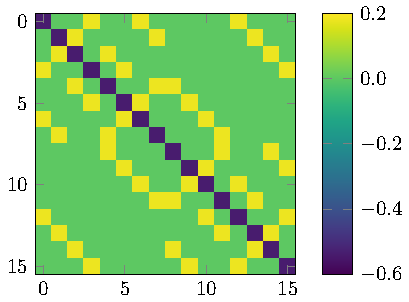
\includegraphics[width=.6\linewidth]{matrix.pdf}
    \caption{Graphical representation of the term $\Fc_{(2)}$ for the time-dependent generator $\Fc_t$ of the Ising spin chain model.}
    \label{fig:matrix}
\end{figure}

Numerically, we verified that $\Fc_{(1)}=\Fc_{(3)}=0$ while $\Fc_{(2)}$ is graphically represented in Fig. \ref{fig:matrix} where one can verify that $\Fc_{(2)}$ is Metzler (i.e. A matrix $A$ is Metzler if $A_{i,j}\geq0$ for all $i\neq j$) and is such that $\onev^T \Fc_{(2)} = 0$. Those two conditions are the classical equivalent to the properties characterizing a Lindblad generator and in fact imply that $e^{\Fc_{(2)}t}$ is a stochastic matrix for all $t\geq0$. This directly implies that $\Tb e^{\int_0^t \Fc_{s,2} ds}$ is CPTP, or stochastic in this case, for all $t\geq0$. 

Fig. \ref{fig:spin_chain} shows the results of the simulations of the Ising spin chain model with $N_B = 4$, $A= 0.3$, $h=0.36$ where we can observe similar results to the other simulations included in this work: increasing the approximation degree decreases the error $\norm{\eta_t-\mu_t}_2$ at low times; for $N=2$ the approximate evolved state $\mu_t$ remains a probability distribution while for $N\geq4$, after a certain time, the state is no longer a probability distribution. 

 

\section{Conclusions and outlook}
\label{sec:conclusion}

\TG{ Pros of the method: 1) The method is iterative and can thus be easily tested (implemented) for small system's sizes. 2) Does not require moving to a rotating frame. 3) The method does not only work for Hamiltonian methods but also includes Lindbladian evolutions. 4) The approach is very general and does not only include the 

Cons of the method: 1) The method only works for short-time approximations. 

Outlook:
\begin{itemize}
    \item convergence of the considered series (lifting part Assumption 2 to get from polynomial to analytic). Say it can be interesting mathematically but practically one would not want to do it. Also explain the difficulties we could encounter (proof of thm1).
    \item What happens if we remove the assumption $\Pc(\rho_0)= \rho_0$
\end{itemize}}

\section{Code availability}
The code necessary to reproduce all the numerical experiments presented in this work is available at \cite{Myrepo}. 

\section{Acknowledgments}
The author would like to thank Francesco Ticozzi for his contribution in the primordial idea of this work and for his constant support. The author would also like to thank Lorenza Viola, Michiel Burgelman and Augusto Ferrante for the useful discussions on the matters of this work. 

\bibliography{ref}

\onecolumngrid
\appendix

\section{Technical results and proofs}
\subsection{Time-ordered expansion} 
\label{sec:thechnical_results:time_ordered}
Before proving the main result, Theorem \ref{thm:time_ordered_expansion}, we shall develop some intuition about how we prove it.
\begin{example}
To provide some intuition about Theorem \ref{thm:time_ordered_expansion} let us consider a simple case: \(\Fc_t = \Fc_{(1)} + t \Fc_{(2)} +t^2 \Fc_{(3)}\). 
Let us first compute the first few terms of the Dyson expansion \cite{Dyson} of $\Tb e^{\int_0^t \Fc_s ds}$, i.e. $\Tb e^{\int_0^t \Fc_s ds} = \sum_{n=0}^{+\infty} \Phi_{(n),t}$.
At zeroth order we have $\Phi_{(0),t} = \Ic$ while at orders $1,2$ and $3$ we have:
\begin{align*}
    \Phi_{(1),t} &= \int_0^t \Fc_{s} ds = \int_0^t (\Fc_{(1)} + s\Fc_{(2)} + s^{2} \Fc_{(3)}) ds = 
    t \Fc_{(1)} + t^2\frac{\Fc_{(2)}}{2} + t^3 \frac{\Fc_{(3)}}{3} ,
\end{align*}
\begin{align*}
    \Phi_{(2),t} &= \int_0^t dt_1\, \int_0^{t_1} dt_2\, \Fc_{t_1} \Fc_{t_2} 
    = \sum_{j=0}^{1} \int_0^t dt_1\, \Fc_{t_1} \Fc_{(j+1)} \int_0^{t_1} dt_2\,  t_2^j 
    = \sum_{j=0}^{1} \int_0^t dt_1\, \Fc_{t_1}\Fc_{(j+1)}  \frac{t_1^{j+1}}{j+1}\\
    & = \sum_{k,j=0}^{1} \Fc_{(k+1)}\Fc_{(j+1)} \int_0^t dt_1\, t_1^k \frac{t_1^{j+1}}{j+1} = \sum_{k,j=0}^{1} \Fc_{(k+1)}\Fc_{(j+1)} \frac{t^{k+j+2}}{(k+j+2)(j+1)} = \sum_{k,j=1}^{2} \Fc_{(k)}\Fc_{(j)} \frac{t^{k+j}}{(j+k)j}\\
    &= \underbrace{\Fc_{(1)}^2 \frac{t^2}{2}}_{j=k=1}
    + \underbrace{\Fc_{(2)}\Fc_{(1)}\frac{t^3}{3}}_{j=1,k=2} 
    + \underbrace{\Fc_{(1)}\Fc_{(2)}\frac{t^3}{6}}_{j=2,k=1} 
    %+ \underbrace{\Fc_{(2)}^2 \frac{t^4}{8}}_{j=k=2} 
    + O(t^4),
\end{align*}
\begin{align*}
    \Phi_{(3),t} &= \int_0^t dt_1 \int_0^{t_1} dt_2 \int_0^{t_2} dt_3 \Fc_{t_1} \Fc_{t_2} \Fc_{t_3} = \int_0^t dt_1 \Fc_{t_1} \underbrace{\int_0^{t_1} dt_2 \int_0^{t_2} dt_3  \Fc_{t_2} \Fc_{t_3}}_{= \sum_{j,k=1}^{2} \Fc_{(k)}\Fc_{(j)} \frac{t_1^{k+j}}{(j+k)j}}\\ 
    &= \sum_{h,k,j=1}^{2} \Fc_{(h)}\Fc_{(k)}\Fc_{(j)} \int_0^t dt_1\, t_1^h \frac{t_1^{k+j}}{(j+k)j} = \sum_{h,k,j=1}^{2} \Fc_{(h)}\Fc_{(k)}\Fc_{(j)}  \frac{t^{h+k+j}}{(h+k+j)(j+k)j} 
     = \underbrace{\Fc_{(1)}^3 \frac{t^{3}}{3!}}_{h=k=j=1} + O(t^4).
\end{align*}
Grouping together the terms of $\Tb e^{\int_0^t \Fc_s ds}$ by the order of the exponent of $t$, we have 
\begin{align*}
    \Tb e^{\int_0^t \Fc_s ds} &= \underbrace{\Ic}_{\Ec_{(0)}} + t \underbrace{\Fc_{(1)}}_{\Ec_{(1)}} + t^2 \underbrace{\left( \frac{\Fc_{(2)}}{2} + \frac{\Fc_{(1)}^2}{2} \right)}_{\Ec_{(2)}} + t^3 \underbrace{\left(\frac{\Fc_{(3)}}{3}+\frac{\Fc_{(1)}\Fc_{(2)}}{6} +\frac{\Fc_{(2)}\Fc_{(1)}}{3} + \frac{\Fc_{(1)}^3}{3!} \right)}_{\Ec_{(3)}} +O(t^4)
\end{align*}
which coincides with the first few terms obtained using the equation given in Theorem \ref{thm:time_ordered_expansion}:
\begin{align*}
    \Ec_{(0)} &= \Ic,\\
    \Ec_{(1)} &= \Fc_{(1)}\Ec_{(0)} = \Fc_{(1)},\\
    \Ec_{(2)} &= \frac{1}{2}(\Fc_{(1)}\Ec_{(1)} +  \Fc_{(2)}\Ec_{(0)}) = \frac{1}{2}(\Fc_{(1)}^2 + \Fc_{(2)}),\\
    \Ec_{(2)} &= \frac{1}{3}(\Fc_{(1)}\Ec_{(2)} +  \Fc_{(2)}\Ec_{(1)} + \Fc_{(3)}\Ec_{(0)}) = \frac{1}{3}(\frac{1}{2}\Fc_{(1)}^3 + \frac{1}{2}\Fc_{(1)}\Fc_{(2)} + \Fc_{(2)}\Fc_{(1)} +\Fc_{(3)}).
\end{align*}
\end{example}
\begin{proof}[Theorem \ref{thm:time_ordered_expansion}]
    We shall start by proving that $\Tb e^{\int_0^t \Fc_s ds} = \sum_{n=0}^{+\infty} \Phi_{(n),t}$ where $\Phi_{(0,t)} = \Ic$ and, for $n>0$, \[\Phi_{(n),t} = \sum_{k_1,\dots,k_n=1}^{N+1} t^{\sum_{j=1}^n k_j} \frac{ \Fc_{(k_1)} \dots\Fc_{(k_n)}}{\prod_{j=1}^n \sum_{h=n-j+1}^n k_h}.\]
    First of all, using the Dyson series expansion for the time-ordered exponential $\Tb e^{\int_0^t \Fc_s ds}$, see e.g. \cite{Dyson, argeri2014magnus, sakurai2020modern}, we have that: 
    \[\Tb e^{\int_0^t \Fc_s ds} = \sum_{n=0}^{+\infty} \Phi_{(n),t} \qquad\text{ with }\qquad 
    \Phi_{(n),t} = \int_0^t dt_1\, \int_0^{t_1} dt_2\, \dots \int_0^{t_{n-1}} dt_n\, \Fc_{t_1}\Fc_{t_2}\dots\Fc_{t_n}\,    .\]
    Next, by noticing that \(\Phi_{(n),t} = \int_0^t ds\, \Fc_{s} \Phi_{(n-1),s} \) we can prove the statement by induction.
    The case $n=1$ is proven by simple calculations:
    \begin{align*}
        \Phi_{(1),t} &= \int_0^t ds\, \Fc_{s}  = \int_0^t ds\, \sum_{k_1=0}^N s^{k_1}\Fc_{(k_1+1)} = \sum_{k_1=0}^{N} \Fc_{(k_1+1)} \int_0^t ds\, s^{k_1}  
        = \sum_{k_1=0}^{N} \Fc_{(k_1+1)} \frac{t^{k_1+1}}{k_1+1} 
         = \sum_{k_1=1}^{N+1} \Fc_{(k_1)} \frac{t^{k_1}}{k_1}.
    \end{align*}
    Note that $\int_0^t ds \sum_{k=0}^N = \sum_{k=0}^{N} \int_0^t ds$ under the assumption that $N$ is finite, i.e. $N<\infty$. 
    We next assume that the statement holds for $n$, i.e. 
    \[\Phi_{(n),t} = \sum_{k_1,\dots,k_n=1}^{N+1} t^{\sum_{j=1}^n k_j} \frac{\Fc_{(k_1)}\dots\Fc_{(k_n)}}{\prod_{j=1}^n \sum_{h=n-j+1}^n k_h}.\]
    Then 
    \begin{align*}
        \Phi_{(n+1),t} &= \int_0^t ds\, \Fc_s \Phi_{(n),s} 
        = \int_0^t ds\, \Fc_s \sum_{k_1,\dots,k_n=1}^{N+1} s^{\sum_{j=1}^n k_j} \frac{ \Fc_{(k_n)}\dots\Fc_{(k_1)}}{\prod_{j=1}^n \sum_{h=n-j+1}^n k_h} \\
        &= \int_0^t ds\, \sum_{k=0}^{N} s^k \Fc_{(k+1)} \sum_{k_1,\dots,k_n=1}^{N+1}  s^{\sum_{j=1}^n k_j} \frac{ \Fc_{(k_1)} \dots \Fc_{(k_n)}}{\prod_{j=1}^n \sum_{h=n-j+1}^n k_h} \\
        &= \sum_{k=0}^{N} \sum_{k_1,\dots,k_n=1}^{N+1} \Fc_{(k+1)} \frac{ \Fc_{(k_1)}\dots\Fc_{(k_n)}}{\prod_{j=1}^n \sum_{h=n-j+1}^n k_h}  \int_0^t s^{k+\sum_{j=1}^n k_j} ds \\
        &= \sum_{k=0}^{N} \sum_{k_1,\dots,k_n=1}^{N+1} \frac{t^{k+1+\sum_{j=1}^n k_j}}{k+1+\sum_{j=1}^n k_j} \Fc_{(k+1)} \frac{\Fc_{(k_1)}\dots\Fc_{(k_n)}}{\prod_{j=1}^n \sum_{h=n-j+1}^n k_h} \\
        &= \sum_{k=1}^{N+1} \sum_{k_1,\dots,k_n=1}^{N+1} \frac{t^{k+\sum_{j=1}^n k_j}}{k+\sum_{j=1}^n k_j} \Fc_{(k)} \frac{\Fc_{(k_1)}\dots\Fc_{(k_n)}}{\prod_{j=1}^n \sum_{h=n-j+1}^n k_h} \\
        &= \sum_{k_1=1}^{N+1} \sum_{k_2,\dots,k_{n+1}=1}^{N+1} \frac{t^{k_1+\sum_{j=2}^{n+1} k_j}}{k_1+\sum_{j=2}^{n+1} k_j} \frac{\Fc_{(k_1)}\Fc_{(k_2)}\dots\Fc_{(k_{n+1})}}{\prod_{j=1}^{n} \sum_{h=n-j+2}^{n+1} k_h}\\
        &= \sum_{k_1,\dots,k_{n+1}=1}^{N+1} \frac{t^{\sum_{j=1}^{n+1} k_j}}{\sum_{j=1}^{n+1} k_j} \frac{\Fc_{(k_1)}\dots\Fc_{(k_{n+1})}}{\prod_{j=1}^{n} \sum_{h=n-j+2}^{n+1} k_h}\\
        &= \sum_{k_1,\dots,k_{n+1}=1}^{N+1} t^{\sum_{j=1}^{n+1} k_j} \frac{\Fc_{(k_1)}\dots\Fc_{(k_{n+1})}}{\prod_{j=1}^{n+1} \sum_{h=n-j+2}^{n+1} k_h}.
    \end{align*}
    thus proving the statement.
    
    % \TG{The technical reason why we choose to assume $N<\infty$ is because in this proof we used in a couple of instances the property that $\int_0^t \sum_{k=0}^N s^k \Fc_{(k+1)} ds = \sum_{k=0}^N \int_0^t s^k \Fc_{(k+1)} ds $ which trivially holds if $N<\infty$. To lift this assumption we would need to assume some extra properties about the superoperators $\Fc_{(k+1)}$.} 

    We next prove that \(\Tb e^{\int_0^t \Fc_s ds} = \sum_{f=0}^{+\infty} t^k \Ec_{(k)}\) where $\Ec_{(0)} = \Ic$ and, for $k>0$,
    \[ \Ec_{(k)} = \sum_{n=1}^k \sum_{\substack{{k_1,\dots,k_{n} = 1}\\{\text{s.t. }\sum_{j=1}^{n}k_{j}=k}}}^{k} \frac{\Fc_{(k_1)}\dots\Fc_{(k_n)} }{\prod_{j=1}^n \sum_{h=n-j+1}^n k_h}. \]
    To prove this claim we can start by noticing that each term $\Phi_{(n),t}$ contains powers $t^k$ of order $k\geq n$. Hence, to construct $\Ec_{(k)}$ of order $k$ we need to collect and sum all the coefficients that multiply $t^k$ among the terms $\Phi_{(n),t}$ for $1\leq n\leq k$. Given $\Phi_{(n),t}$ with $n\leq k$ we have that the coefficient multiplying $t^k$ must satisfy the constraint $\sum_{j=1}^n k_j = k$. 
    Thus, the coefficient of $\Phi_{(n),t}$ that multiply $t^k$ are
    \[\sum_{\substack{{k_1,\dots,k_{n} = 1}\\{\text{s.t. }\sum_{j=1}^{n}k_{j}=k}}}^{N+1} \frac{ \Fc_{(k_1)}\dots\Fc_{(k_n)}}{\prod_{j=1}^n \sum_{h=n-j+1}^n k_h} = \sum_{\substack{{k_1,\dots,k_{n} = 1}\\{\text{s.t. }\sum_{j=1}^{n}k_{j}=k}}}^{k} \frac{ \Fc_{(k_1)}\dots\Fc_{(k_n)}}{\prod_{j=1}^n \sum_{h=n-j+1}^n k_h}\]
    where we used the fact that, if any $k_j>k$ then $\sum_{j=1}^n k_j>k$.  
    Noticing that $\prod_{j=1}^n \sum_{h=n-j+1}^n k_h = k(\prod_{j=1}^{n-1} \sum_{h=n-j+1}^n k_h)$ and summing over $1\leq n\leq k$ we obtain, for $k>0$, the second claim, i.e.  
    \[\Ec_{(k)} = \sum_{n=1}^{k} \sum_{\substack{{k_1,\dots,k_{n} = 1}\\{\text{s.t. }\sum_{j=1}^{n}k_{j}=k}}}^{k} \frac{ \Fc_{(k_1)}\dots\Fc_{(k_n)}}{k(\prod_{j=1}^{n-1} \sum_{h=n-j+1}^n k_h)}.\]

    We are now finally ready to prove the main claim of the theorem, that is: \(\Ec_{(k)} = \frac{1}{k}\sum_{s=1}^{k}\Fc_{(s)}\Ec_{(k-s)}.\)
    Recalling that $\Ec_{(0)}=\Ic$ we can write:
    \begin{align*}
        \frac{1}{k}\sum_{s=1}^{k} \Fc_{(s)} \Ec_{(k-s)}  &= \sum_{s=1}^{k-1} \frac{\Fc_{(s)}}{k} \Ec_{(k-s)} + \frac{\Fc_{(k)}}{k} \\
        &= \sum_{s=1}^{k-1} \sum_{n=1}^{k-s} \sum_{\substack{{k_1,\dots,k_{n} = 1}\\{\text{s.t. }\sum_{j=1}^{n}k_{j}=k-s}}}^{k} \frac{\Fc_{(s)}}{k} \frac{ \Fc_{(k_1)}\dots\Fc_{(k_n)}}{(k-s)(\prod_{j=1}^{n-1} \sum_{h=n-j+1}^n k_h)} + \frac{\Fc_{(k)}}{k} \\
        &= \sum_{s=1}^{k-1}\sum_{n=1}^{k-1} \sum_{\substack{{k_1,\dots,k_{n} = 1}\\{\text{s.t. }\sum_{j=1}^{n}k_{j}=k-s}}}^{k} \frac{\Fc_{(s)}}{k} \frac{ \Fc_{(k_1)}\dots\Fc_{(k_n)}}{(k-s)(\prod_{j=1}^{n-1} \sum_{h=n-j+1}^n k_h)} + \frac{\Fc_{(k)}}{k}  
    \end{align*}
    where we used the fact that $\sum_{n=k-s+1}^{k-1} \sum_{\substack{{k_1,\dots,k_{n} = 1}\\{\text{s.t. }\sum_{j=1}^{n}k_{j}=k-s}}}^{k} \frac{\Fc_{(s)}}{k} \frac{ \Fc_{(k_1)}\dots\Fc_{(k_n)}}{(k-s)(\prod_{j=1}^{n-1} \sum_{h=n-j+1}^n k_h)} = 0$ since for $n>k-s$ we have that $\sum_{j=1}^{n}k_{j} > k-s$ for any set of $k_j$. This implies that
    \begin{align*}
        \frac{1}{k}\sum_{s=1}^{k} \Fc_{(s)}\Ec_{(k-s)}  
        &= \sum_{n=1}^{k} \sum_{s=1}^{k-1} \sum_{\substack{{k_1,\dots,k_{n} = 1}\\{\text{s.t. }\sum_{j=1}^{n}k_{j}=k-s}}}^{k} \frac{\Fc_{(s)}}{k} \frac{ \Fc_{(k_1)}\dots\Fc_{(k_n)}}{(k-s)(\prod_{j=1}^{n-1} \sum_{h=n-j+1}^n k_h)} +\frac{\Fc_{(k)}}{k} \\
        &= \sum_{n=1}^{k-1} \sum_{k_1=1}^{k-1} \sum_{\substack{{k_2,\dots,k_{n+1} = 1}\\{\text{s.t. }\sum_{j=2}^{n+1}k_{j}=k-k_1}}}^{k} \frac{\Fc_{(k_1)}}{k} \frac{ \Fc_{(k_2)}\dots\Fc_{(k_{n+1})}}{\underbrace{(k-k_1)}_{\sum_{h=2}^{n+1}k_h}(\prod_{j=1}^{n-1} \sum_{h=n-j+1}^n k_{h+1})} +\frac{\Fc_{(k)}}{k} \\
        &= \sum_{n=1}^{k-1} \sum_{k_1=1}^{k-1} \sum_{\substack{{k_2,\dots,k_{n+1} = 1}\\{\text{s.t. }\sum_{j=1}^{n+1}k_{j}=k}}}^{k} \frac{\Fc_{(k_1)} \Fc_{(k_2)}\dots\Fc_{(k_{n+1})}}{k(\prod_{j=1}^{n} \sum_{h=n-j+2}^{n+1} k_{h})} +\frac{\Fc_{(k)}}{k} \\
        &= \sum_{n=2}^{k} \sum_{k_1=1}^{k-1} \sum_{\substack{{k_2,\dots,k_{n} = 1}\\{\text{s.t. }\sum_{j=1}^{n}k_{j}=k}}}^{k} \frac{\Fc_{(k_1)} \Fc_{(k_2)}\dots\Fc_{(k_{n})}}{k(\prod_{j=1}^{n-1} \sum_{h=n-j+1}^{n} k_{h})}+\frac{\Fc_{(k)}}{k}\\
        &= \sum_{n=1}^{k} \sum_{k_1=1}^{k} \sum_{\substack{{k_2,\dots,k_{n} = 1}\\{\text{s.t. }\sum_{j=1}^{n}k_{j}=k}}}^{k} \frac{\Fc_{(k_1)} \Fc_{(k_2)}\dots\Fc_{(k_{n})}}{k(\prod_{j=1}^{n-1} \sum_{h=n-j+1}^{n} k_{h})} = \Ec_{(k)},
    \end{align*}    
    thus concluding the proof.
\end{proof}

\section{Calculations for the spin boson model}
\label{sec:spin_boson_model_calculations}
We can write  
\[H = \underbrace{\one_S}_{\equiv S_0} \otimes \underbrace{H_B}_{\equiv E_0} + \underbrace{\sigma_z}_{S_1} \otimes \underbrace{\left(\frac{g}{2}\one + \sum_k \lambda_k b_k + \overline{\lambda}_k b_k^\dag\right)}_{\equiv E_1}\]
so that the second order term becomes $\Fc_{(2)}(\mu) = \sum_{j,k=0}^1 \chi_{j,k}(\rho_B) \left(S_j\mu S_k - \frac{1}{2}\{S_j^\dag S_k, \mu\}\right)$
where $\chi_{j,k}(\rho_B) = \expect{E_k E_j}_B - \expect{E_j}_B \expect{E_k}_B$. 
We can then start by noting that \(\expect{E_1}_B = g/2\) and 
\begin{align*}
    \expect{H_B}_B &= \sum_{k=1}^{N_B} \omega_k \left( \expect{b_k^\dag b_k}_B + \expect{\one}_B/2\right)= \sum_{k=1}^{N_B} \omega_k \left( \frac{1}{e^{\beta \omega_k}-1} + \frac{1}{2}\right) 
    = \sum_{k=1}^{N_B} \frac{\omega_k}{2} \frac{ e^{\beta \omega_k}+1}{e^{\beta \omega_k}-1}
\end{align*} 
in order to compute
\begin{align*}
    \chi_{1,0}(\rho_B) &= \expect{\left(\frac{g}{2}\one + \sum_j\lambda_j b_j + \overline{\lambda}_jb_j^\dag\right)\sum_k\omega_k\left(n_k+\frac{\one}{2}\right)}_B - \frac{g}{2} \expect{H_B}_B\\
    &= \sum_k \frac{g}{2}\omega_k (\expect{n_k}_B + \um) +\sum_{j}\lambda_j\omega_k \cancel{(\expect{b_jn_k}_B +\expect{b_j}_B)} + \overline{\lambda}_j\omega_k\cancel{\left(\expect{b_j^\dag n_k} + \expect{b_j^\dag}_B\right)} - \frac{g}{2} \expect{H_B}_B\\
    & = \sum_k \frac{g}{2}\omega_k \left(\frac{1}{e^{\beta \omega_k}-1} + \um\right) - \frac{g}{2} \frac{\omega_k}{2} \frac{ e^{\beta \omega_k}+1}{e^{\beta \omega_k}-1} = 0
\end{align*}
as $\expect{b_jn_k}_B = \expect{b_j^\dag n_k}_B =0$.

This fact directly implies that $\Fc_{(2)}(\mu) = \sum_{j=0}^1 \chi_{j,j}(\rho_B)\Dc_{S_j}(\mu)$ and, since $S_0=\one_S$ we have that $\Dc_{S_0} = 0$ thus recovering $\Fc_{(2)}(\mu) = \chi_{1,1}(\rho_B)\Dc_{\sigma_z}(\mu)$. It then remains to compute the coefficient
\begin{align*}
    \chi_{1,1}(\rho_B) &= \expect{\left(\frac{g}{2}\one + \sum_k \lambda_k b_k + \overline{\lambda}_k b_k^\dag\right)\left(\frac{g}{2}\one + \sum_k \lambda_k b_k + \overline{\lambda}_k b_k^\dag\right)}_B - \frac{g^2}{4}\\
    &= \cancel{\frac{g^2}{4}\expect{\one}_B} + \sum_k g\left(\lambda_k \cancel{\expect{b_k}_B} + \overline{\lambda}_k \cancel{\expect{b_k^\dag}_B}\right) \\&\qquad +\sum_{j,k} \left(\lambda_j\lambda_k \cancel{\expect{b_jb_k}}_B + \lambda_j\overline{\lambda}_k \expect{b_jb_k^\dag}_B + \overline{\lambda}_j\lambda_k \expect{b_j^\dag b_k}_B + \overline{\lambda_j}\overline{\lambda}_k \cancel{\expect{b_j^\dag b_k^\dag}_B}\right)  - \cancel{\frac{g^2}{4}}\\
    &= \sum_{k=1}^{N_B} \frac{2|\lambda_k|^2}{e^{\beta \omega_k}-1} \equiv \varphi.
\end{align*}

% \clearpage
% \input{old_stuff}
% \clearpage
% \input{open_questions}

\end{document}